\section{设计结果}

\subsection{设计交付物说明}

所提交设计交付物包括图\ref{fig:提交目录结构}所示的比特流文件、不同版本的源代码、性能测试得分,此外还提交了硬件综合设计报告(本报告)的 \LaTeX 源文件及编译得到的 PDF 文件。

\begin{figure}[H]
    \centering
    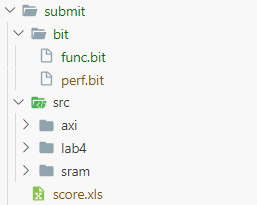
\includegraphics[width=0.5\linewidth]{image/提交目录结构.png}
    \caption{提交目录结构}
    \label{fig:提交目录结构}
\end{figure}

在目录 bit 下包含 AXI 功能测试项目生成的比特流和性能测试项目生成的比特流文件。

在目录 src 下包含三份源代码,分别可用于 lab4 的按指令分类的功能测试、SRAM 接口的功能测试、AXI 接口的功能测试和性能测试。使用时打开对应的 vivado 项目,依次选择 Add Sources、Add or create design sources、Add Directories,在文件目录选择对话框中选择文件夹并添加到项目中。在功能测试或性能测试项目中,为 inst\_ram 选择合适的 coe 文件,点击 Run Simulation 即可运行仿真程序;在性能测试项目中,为 clk\_pll 选择合适的 CPU 时钟频率(本设计中使用的 CPU 时钟频率为 44MHZ),点击 Generate Bitstream 即可生成比特流文件。在 Hardware Manager 中可编程设备并上板测试和查看性能测试得分。

\subsection{设计演示结果}

在答辩环节,现场运行 AXI 接口功能测试仿真程序,观察到控制台输出结果如图\ref{fig:仿真通过}所示。SRAM 接口及 AXI 接口功能测试的 89 个测试点全部通过。

\begin{figure}[H]
    \centering
    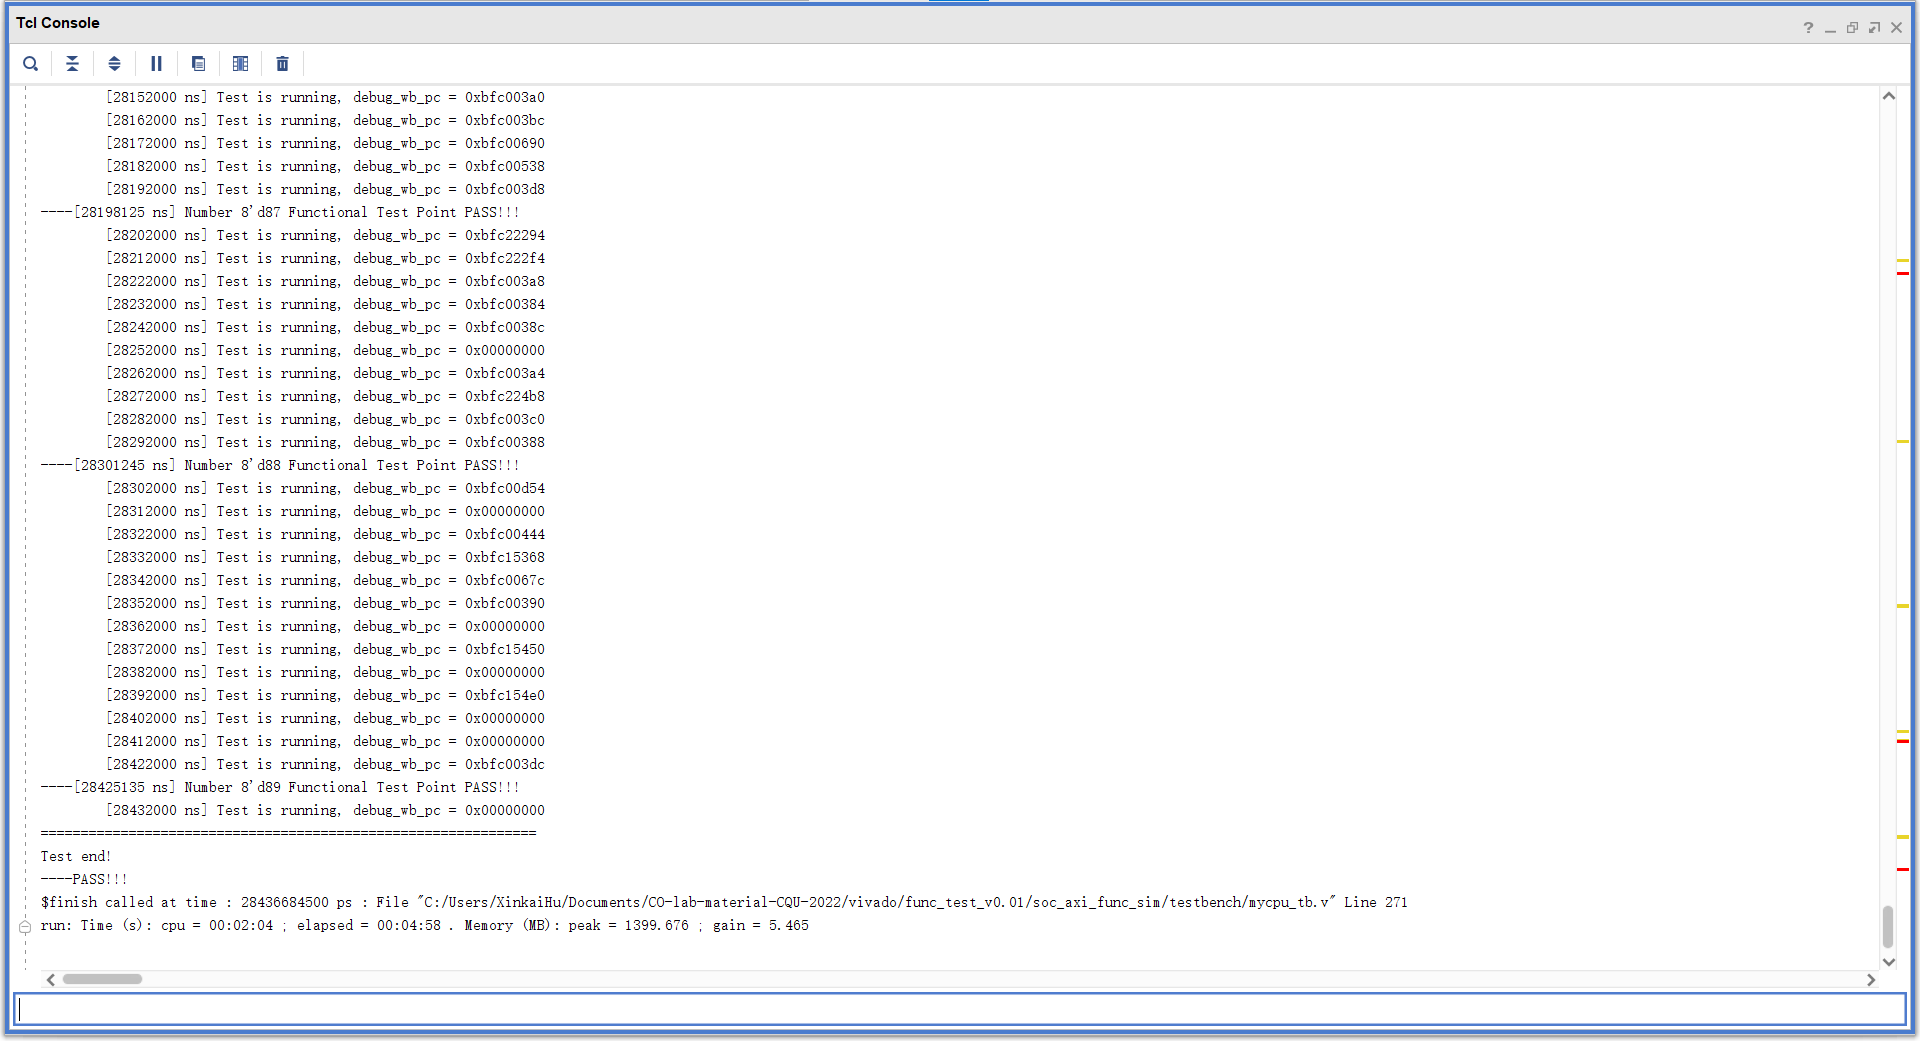
\includegraphics[width=1\linewidth]{image/通过功能测试.png}
    \caption{功能测试运行结果}
    \label{fig:通过功能测试}
\end{figure}

在答辩环节,使用 write-through 直接映射 cache 并将 CPU 时钟频率设置为 44MHZ 后现场生成比特流、上板测试,得到性能测试的得分如下图。性能测试的 10 个测试点全部通过。

\begin{figure}[htbp]
    \centering
    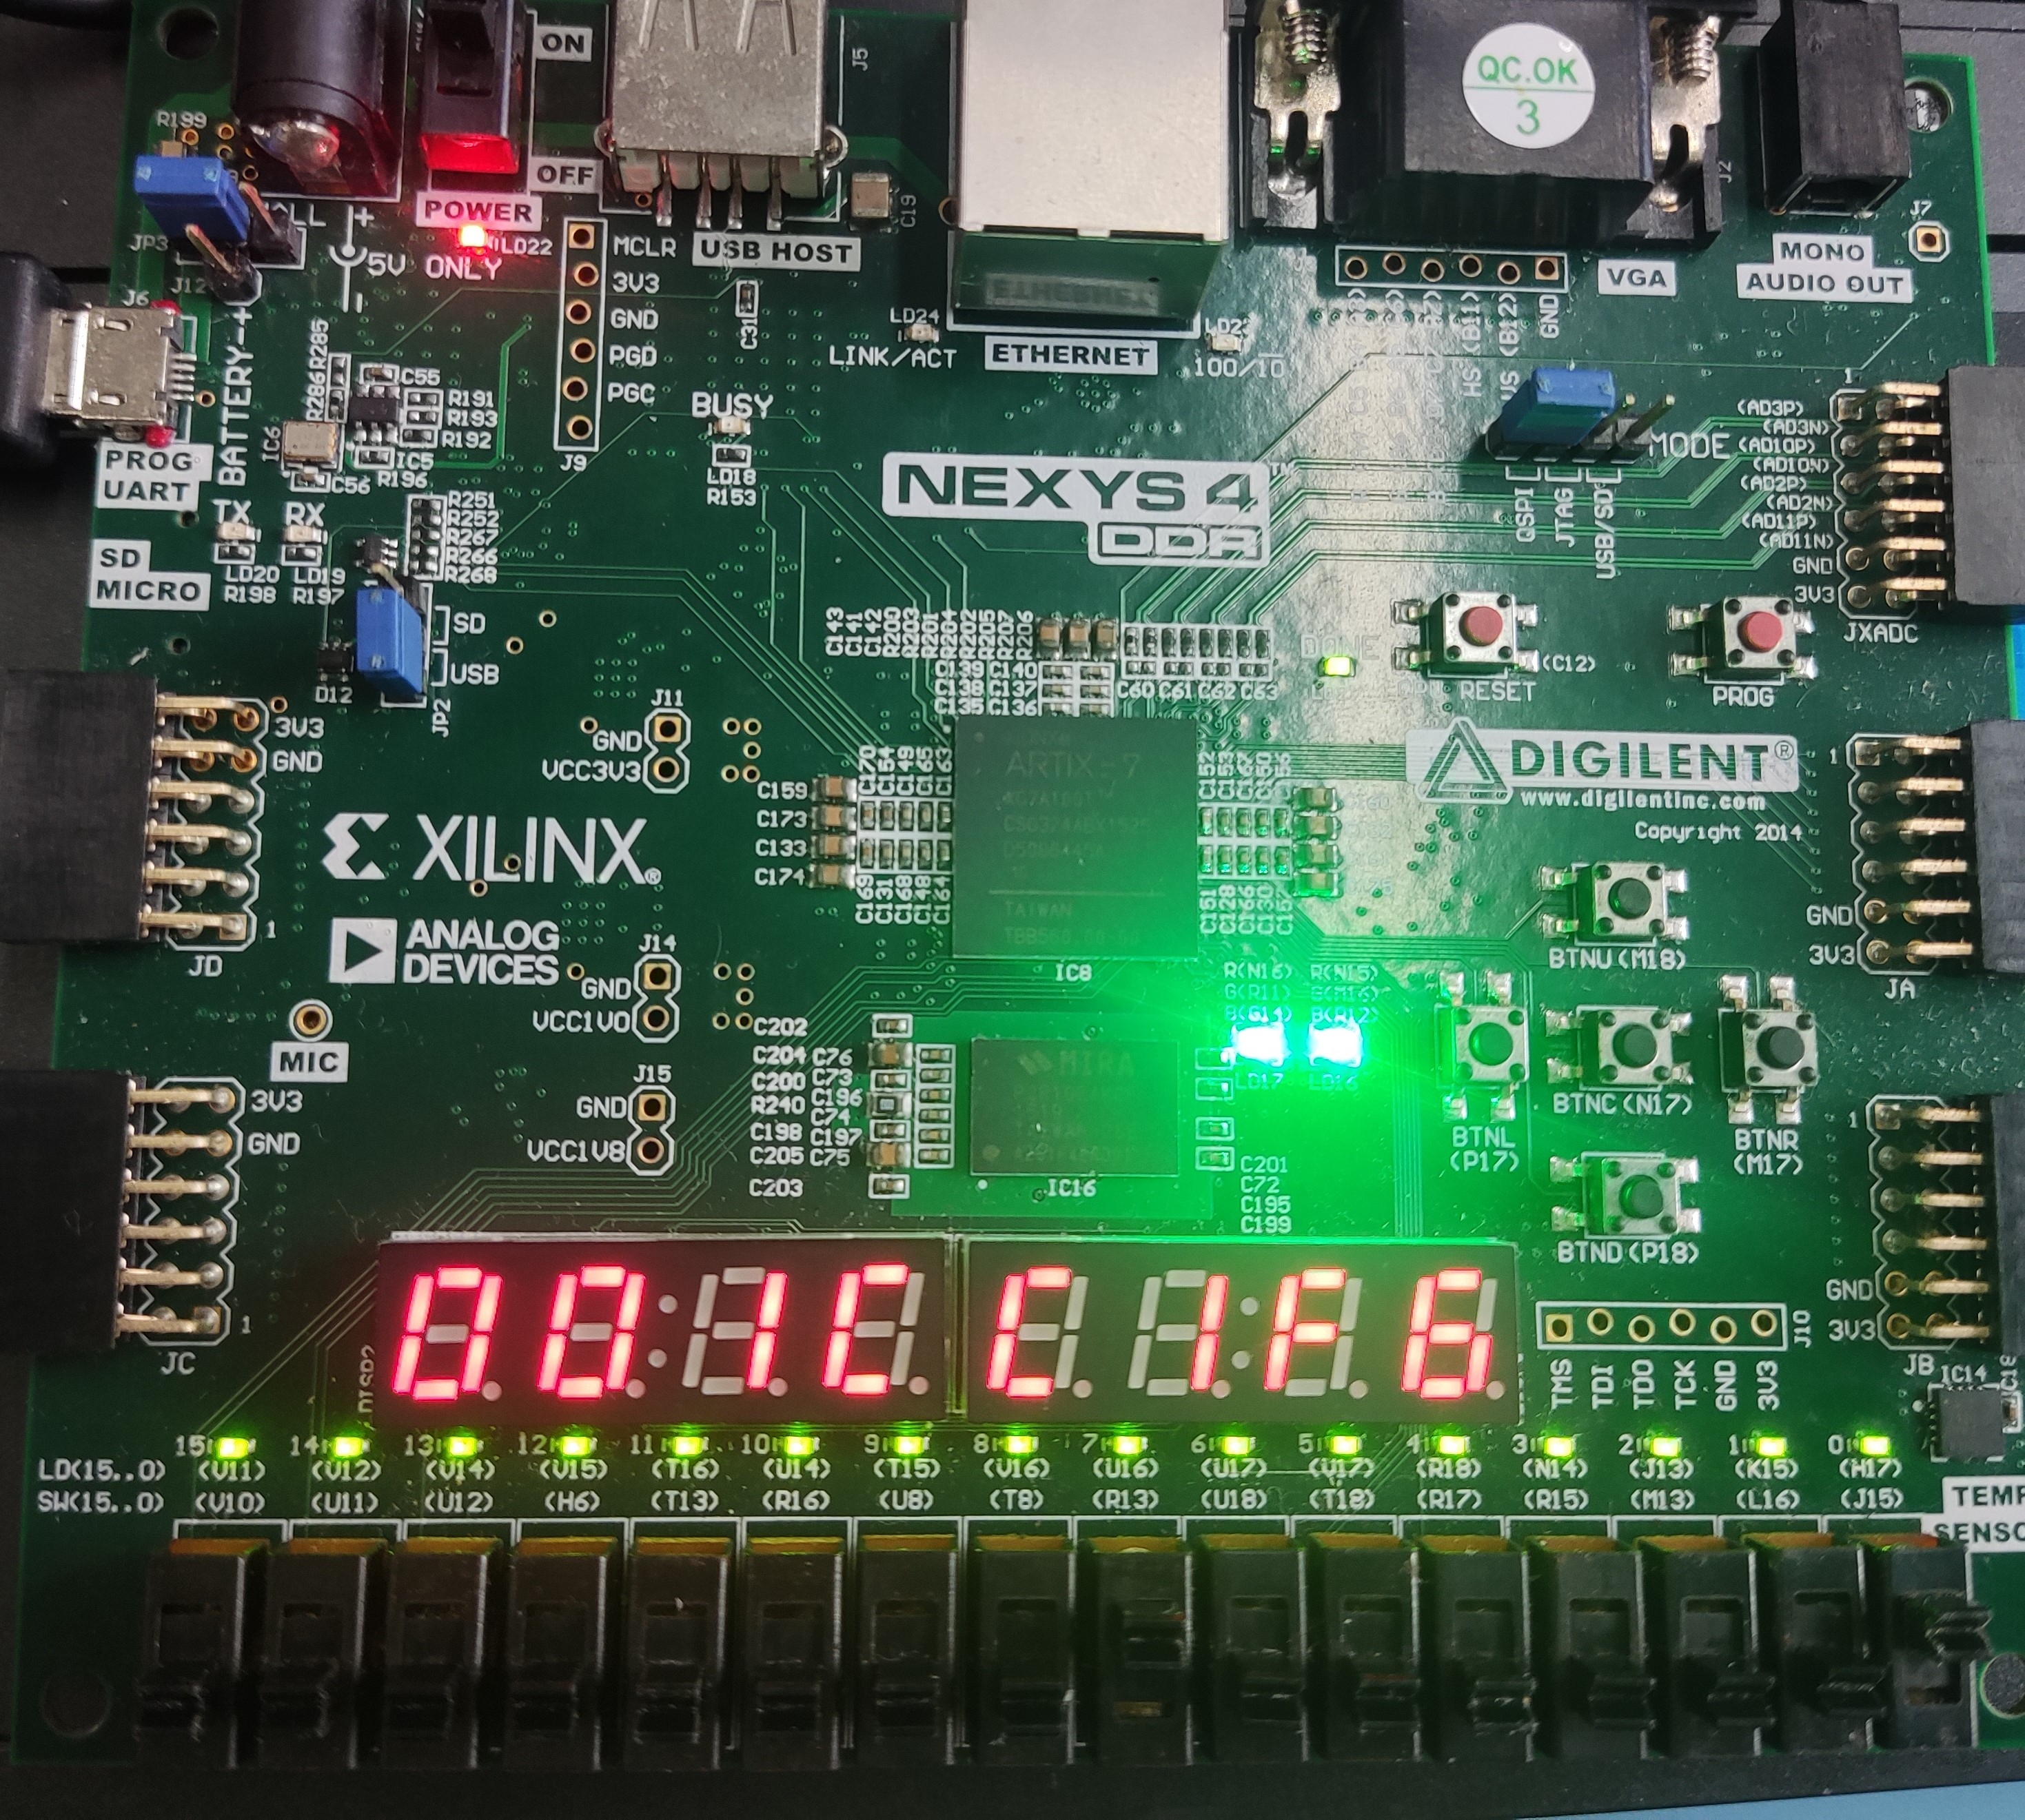
\includegraphics[width=0.7\textwidth]{image/per1.jpg}
    \caption{bitcount 性能测试得分}
    \label{fig:per1}
\end{figure}
\begin{figure}[htbp]
    \centering
    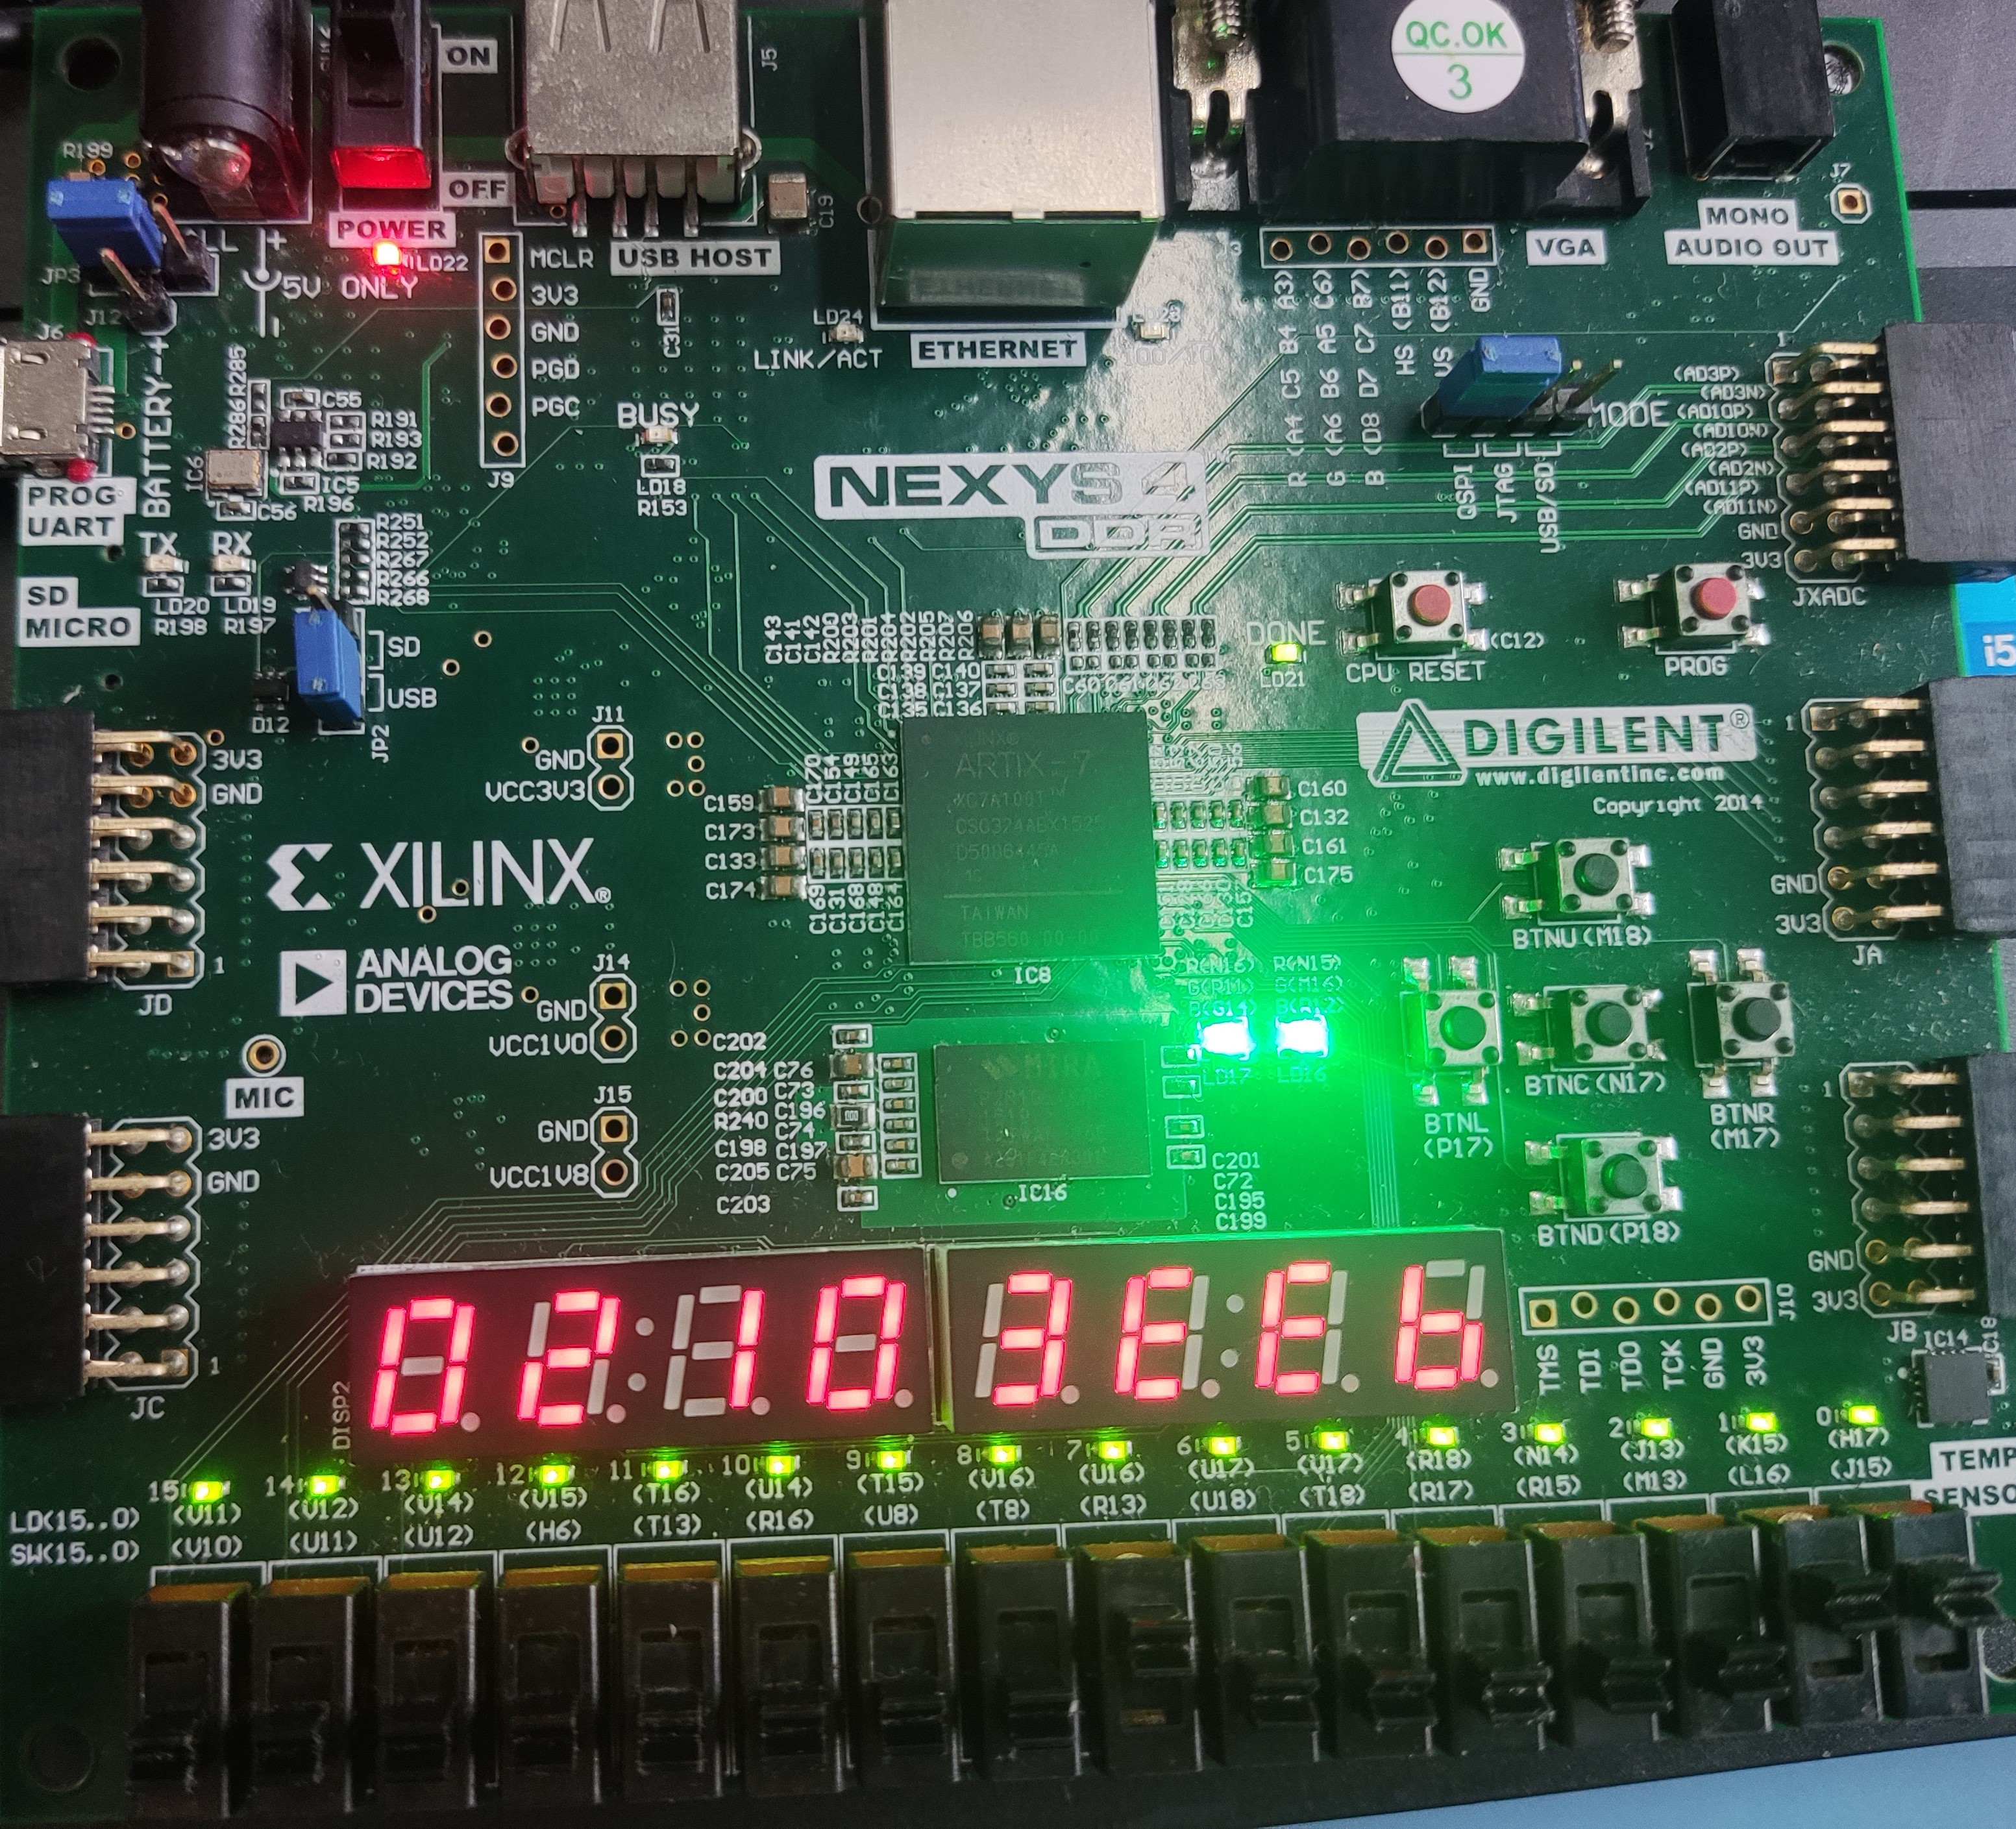
\includegraphics[width=0.7\textwidth]{image/per2.jpg}
    \caption{bubblesort 性能测试得分}
    \label{fig:per2}
\end{figure}
\begin{figure}[htbp]
    \centering
    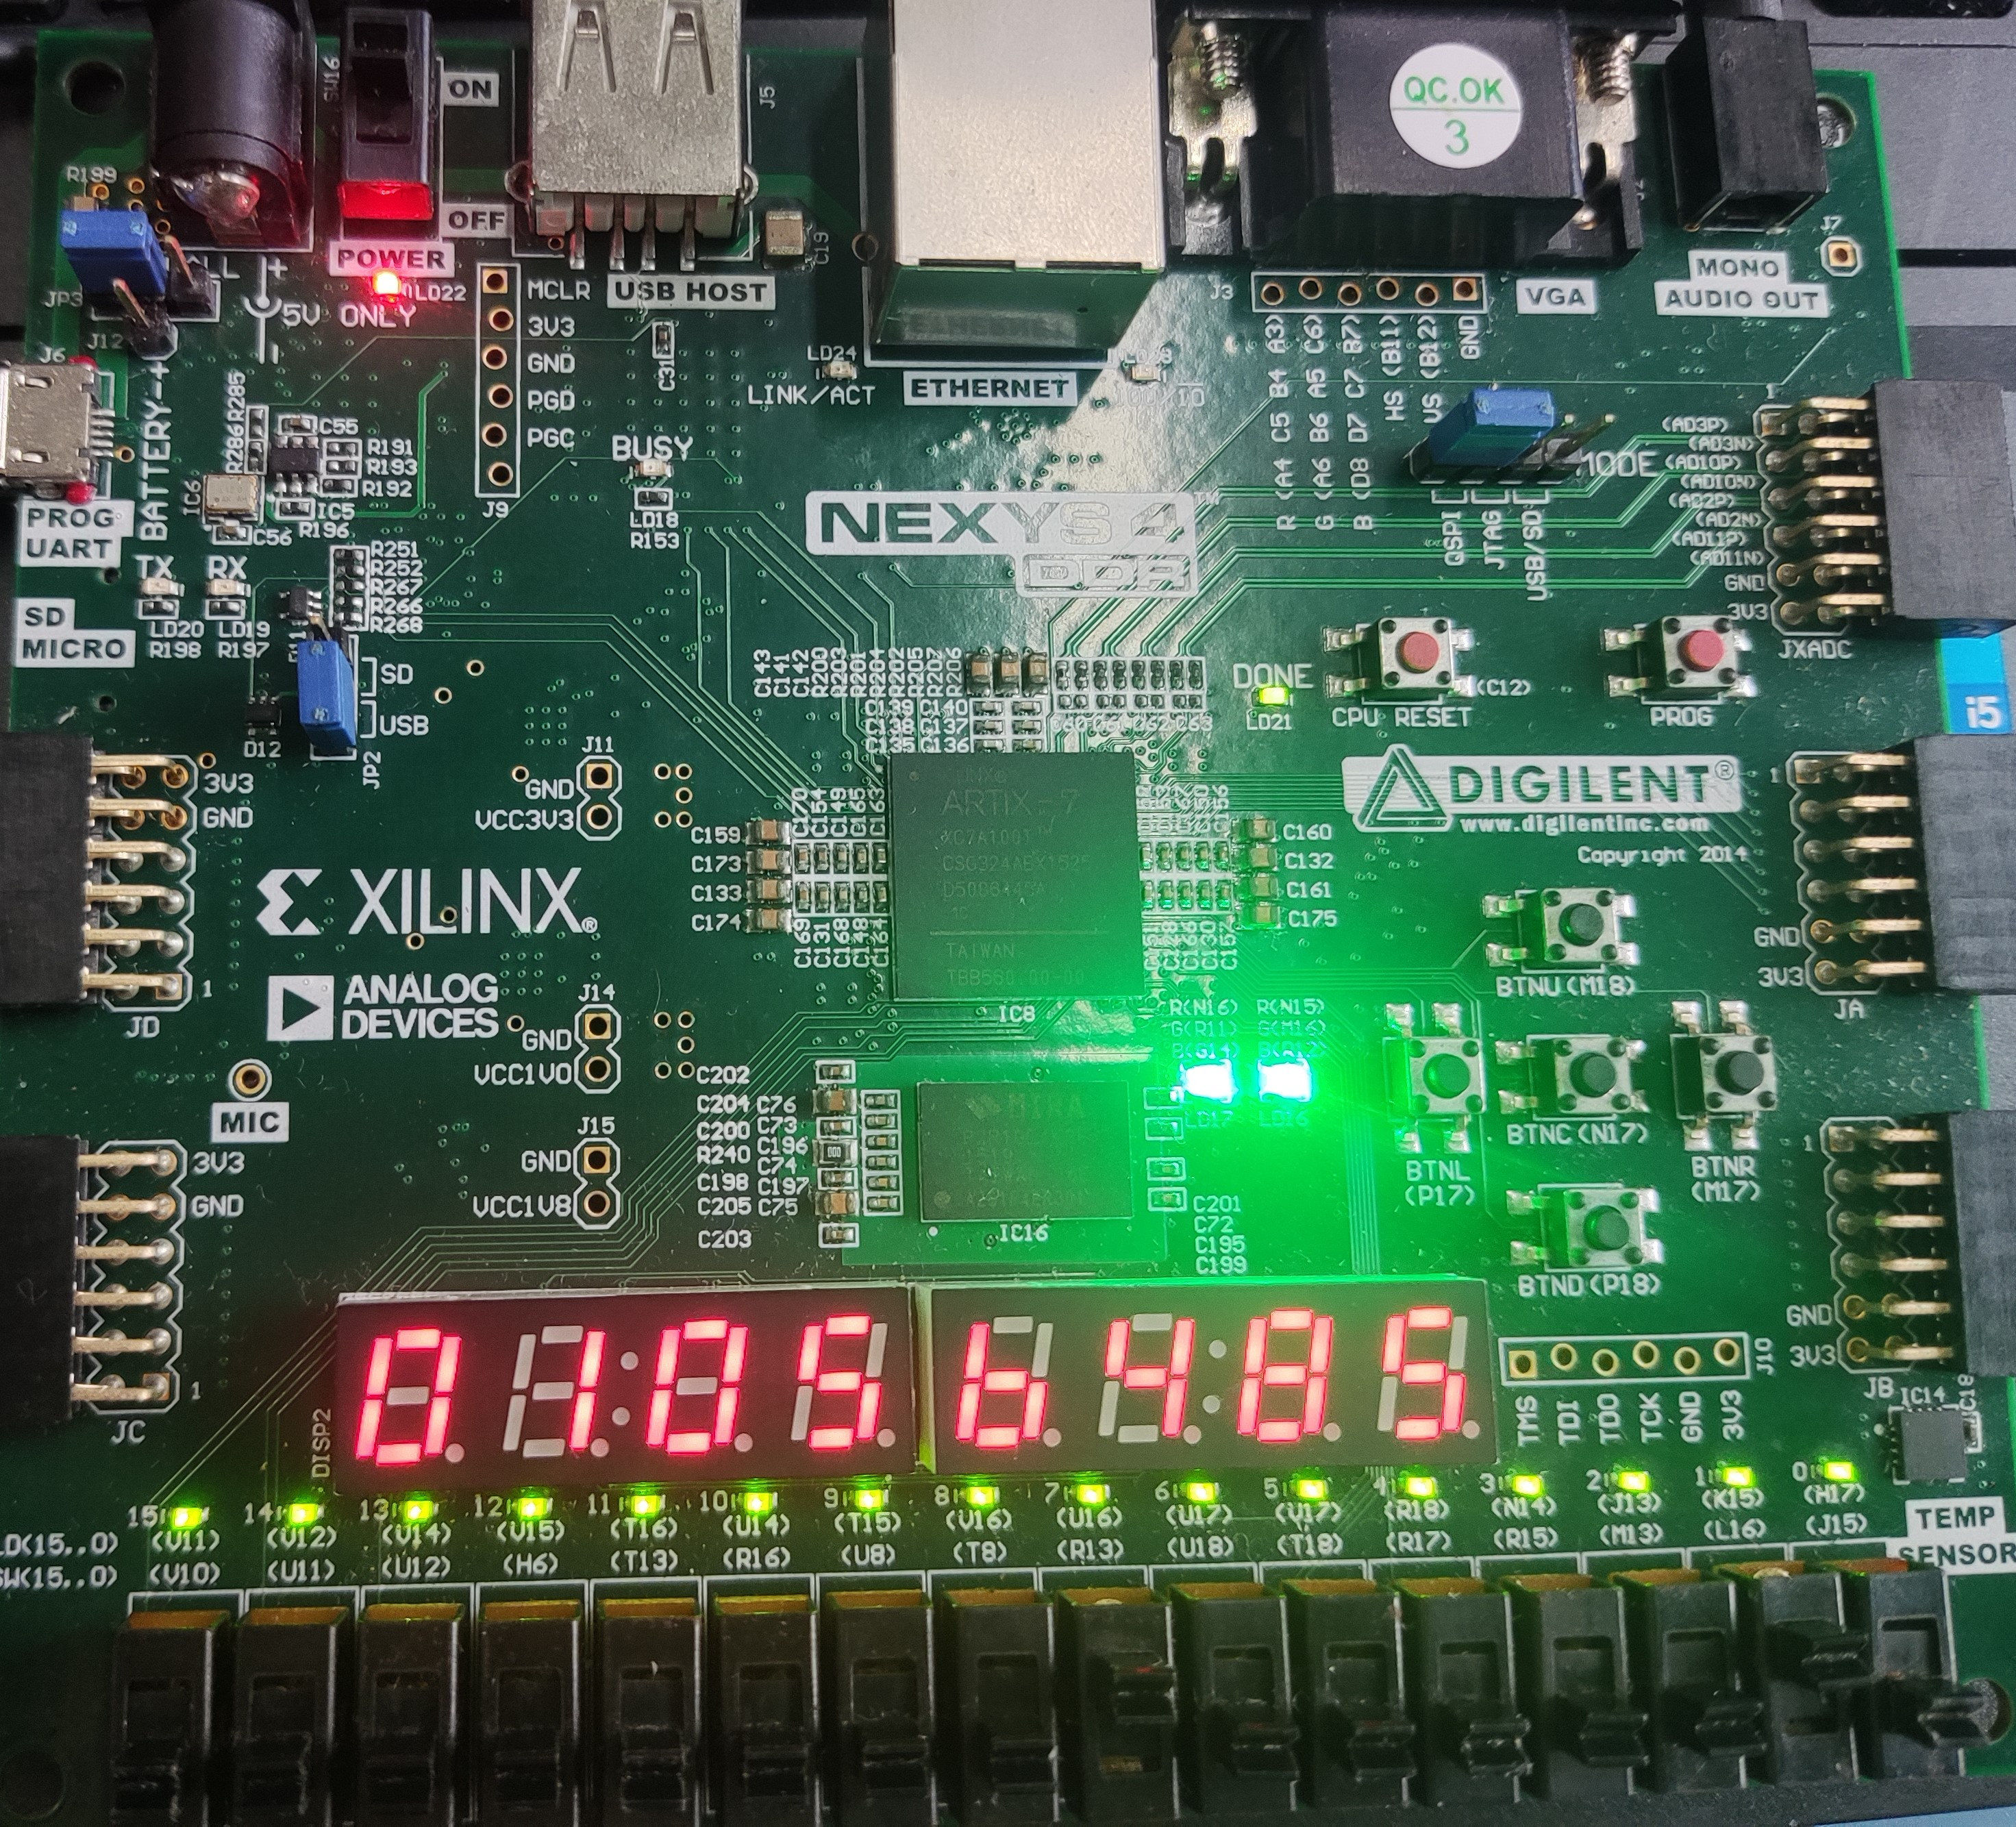
\includegraphics[width=0.7\textwidth]{image/per3.jpg}
    \caption{coremark 性能测试得分}
    \label{fig:per3}
\end{figure}
\begin{figure}[htbp]
    \centering
    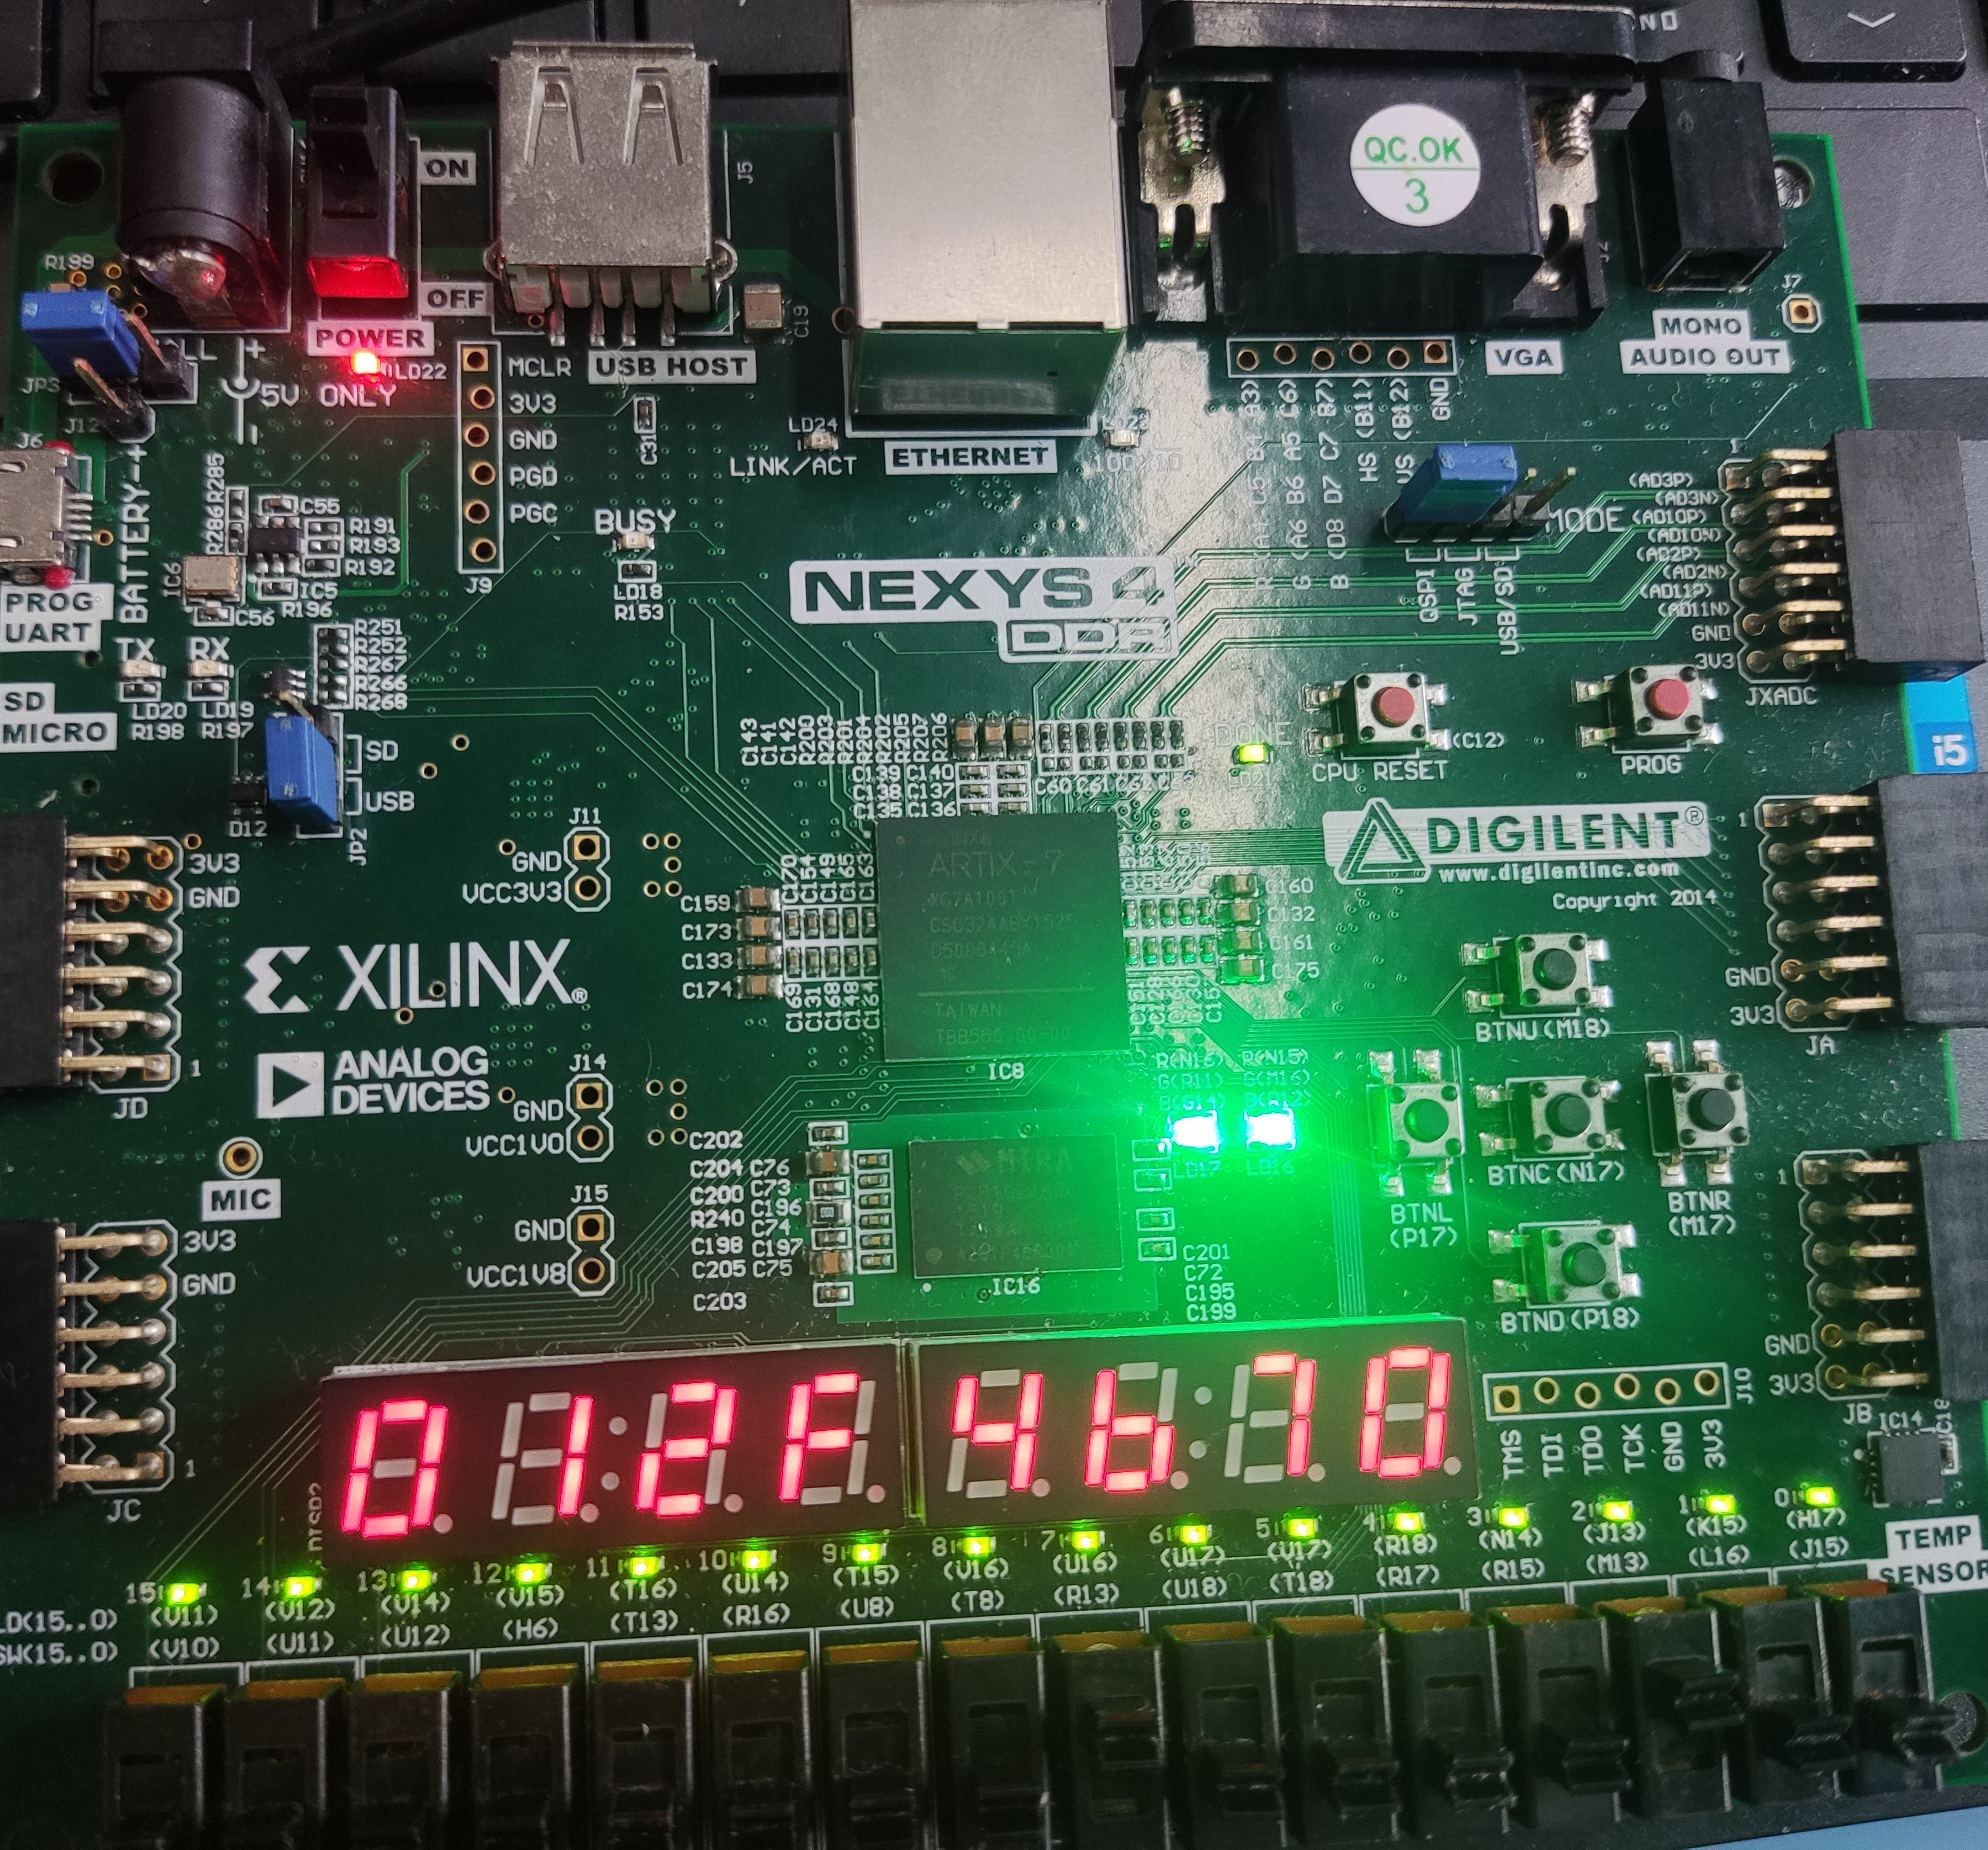
\includegraphics[width=0.7\textwidth]{image/per4.jpg}
    \caption{crc32 性能测试得分}
    \label{fig:per4}
\end{figure}
\begin{figure}[htbp]
    \centering
    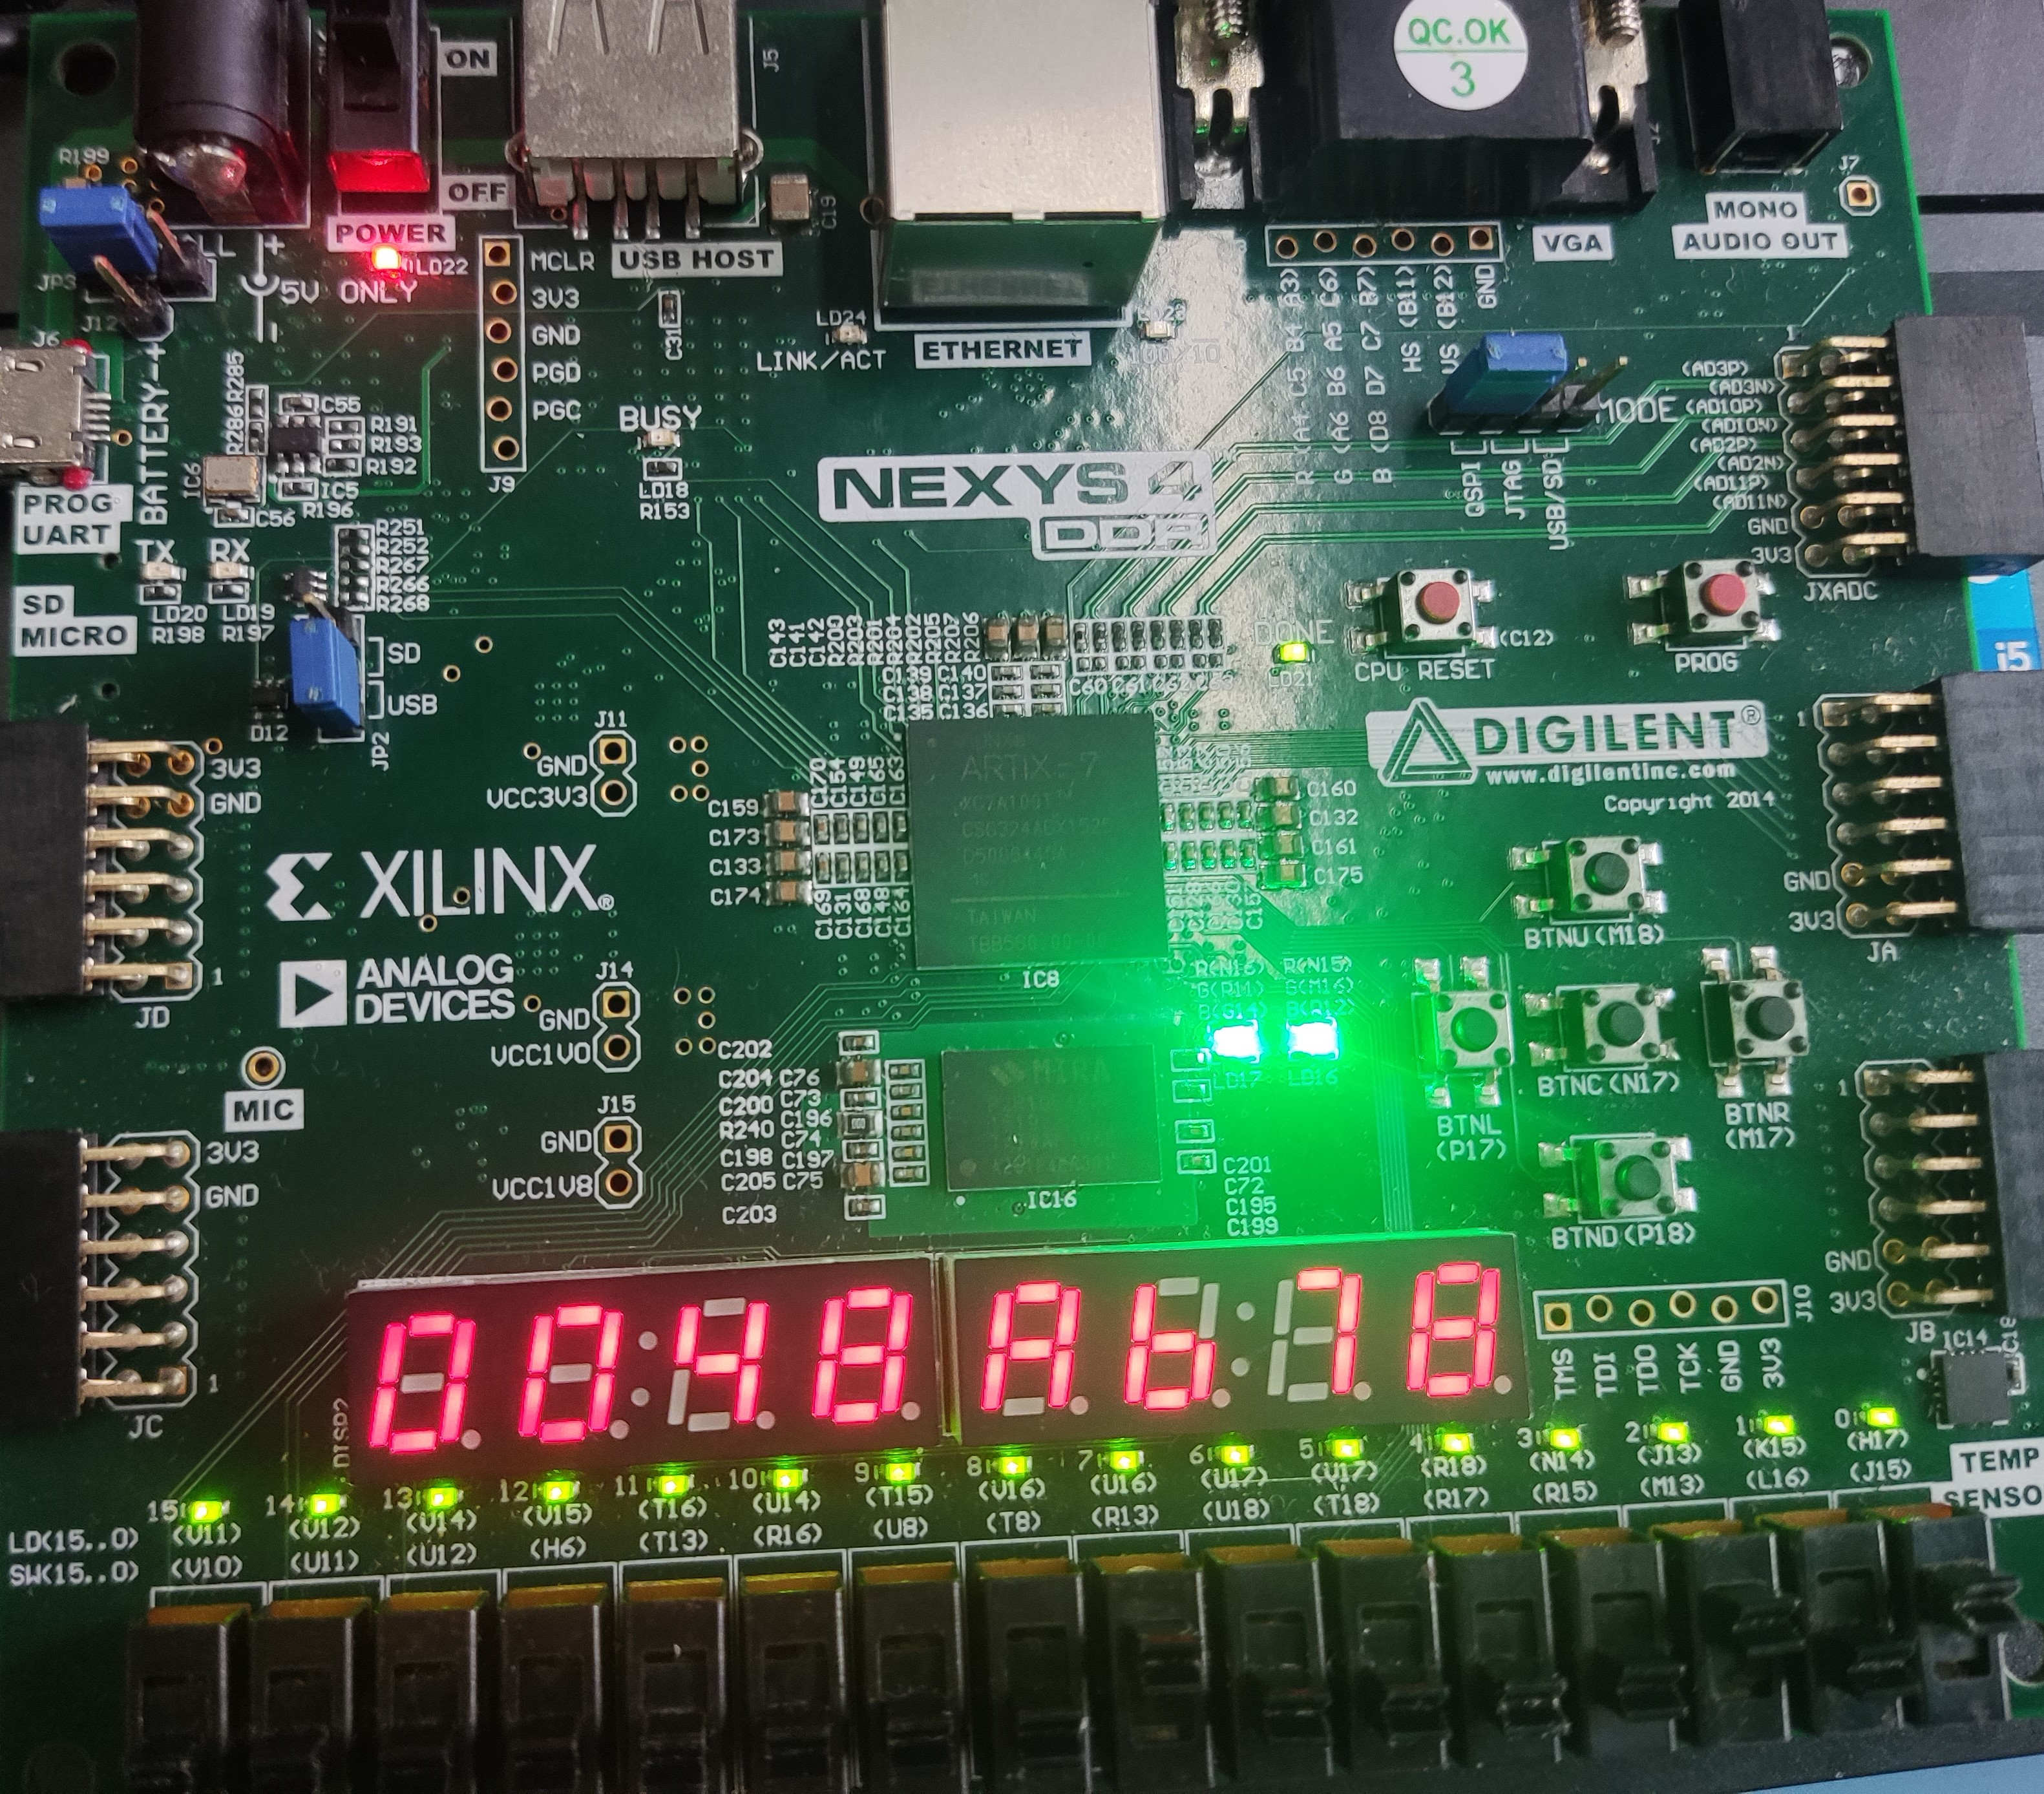
\includegraphics[width=0.7\textwidth]{image/per5.jpg}
    \caption{dhrystone 性能测试得分}
    \label{fig:per5}
\end{figure}
\begin{figure}[htbp]
    \centering
    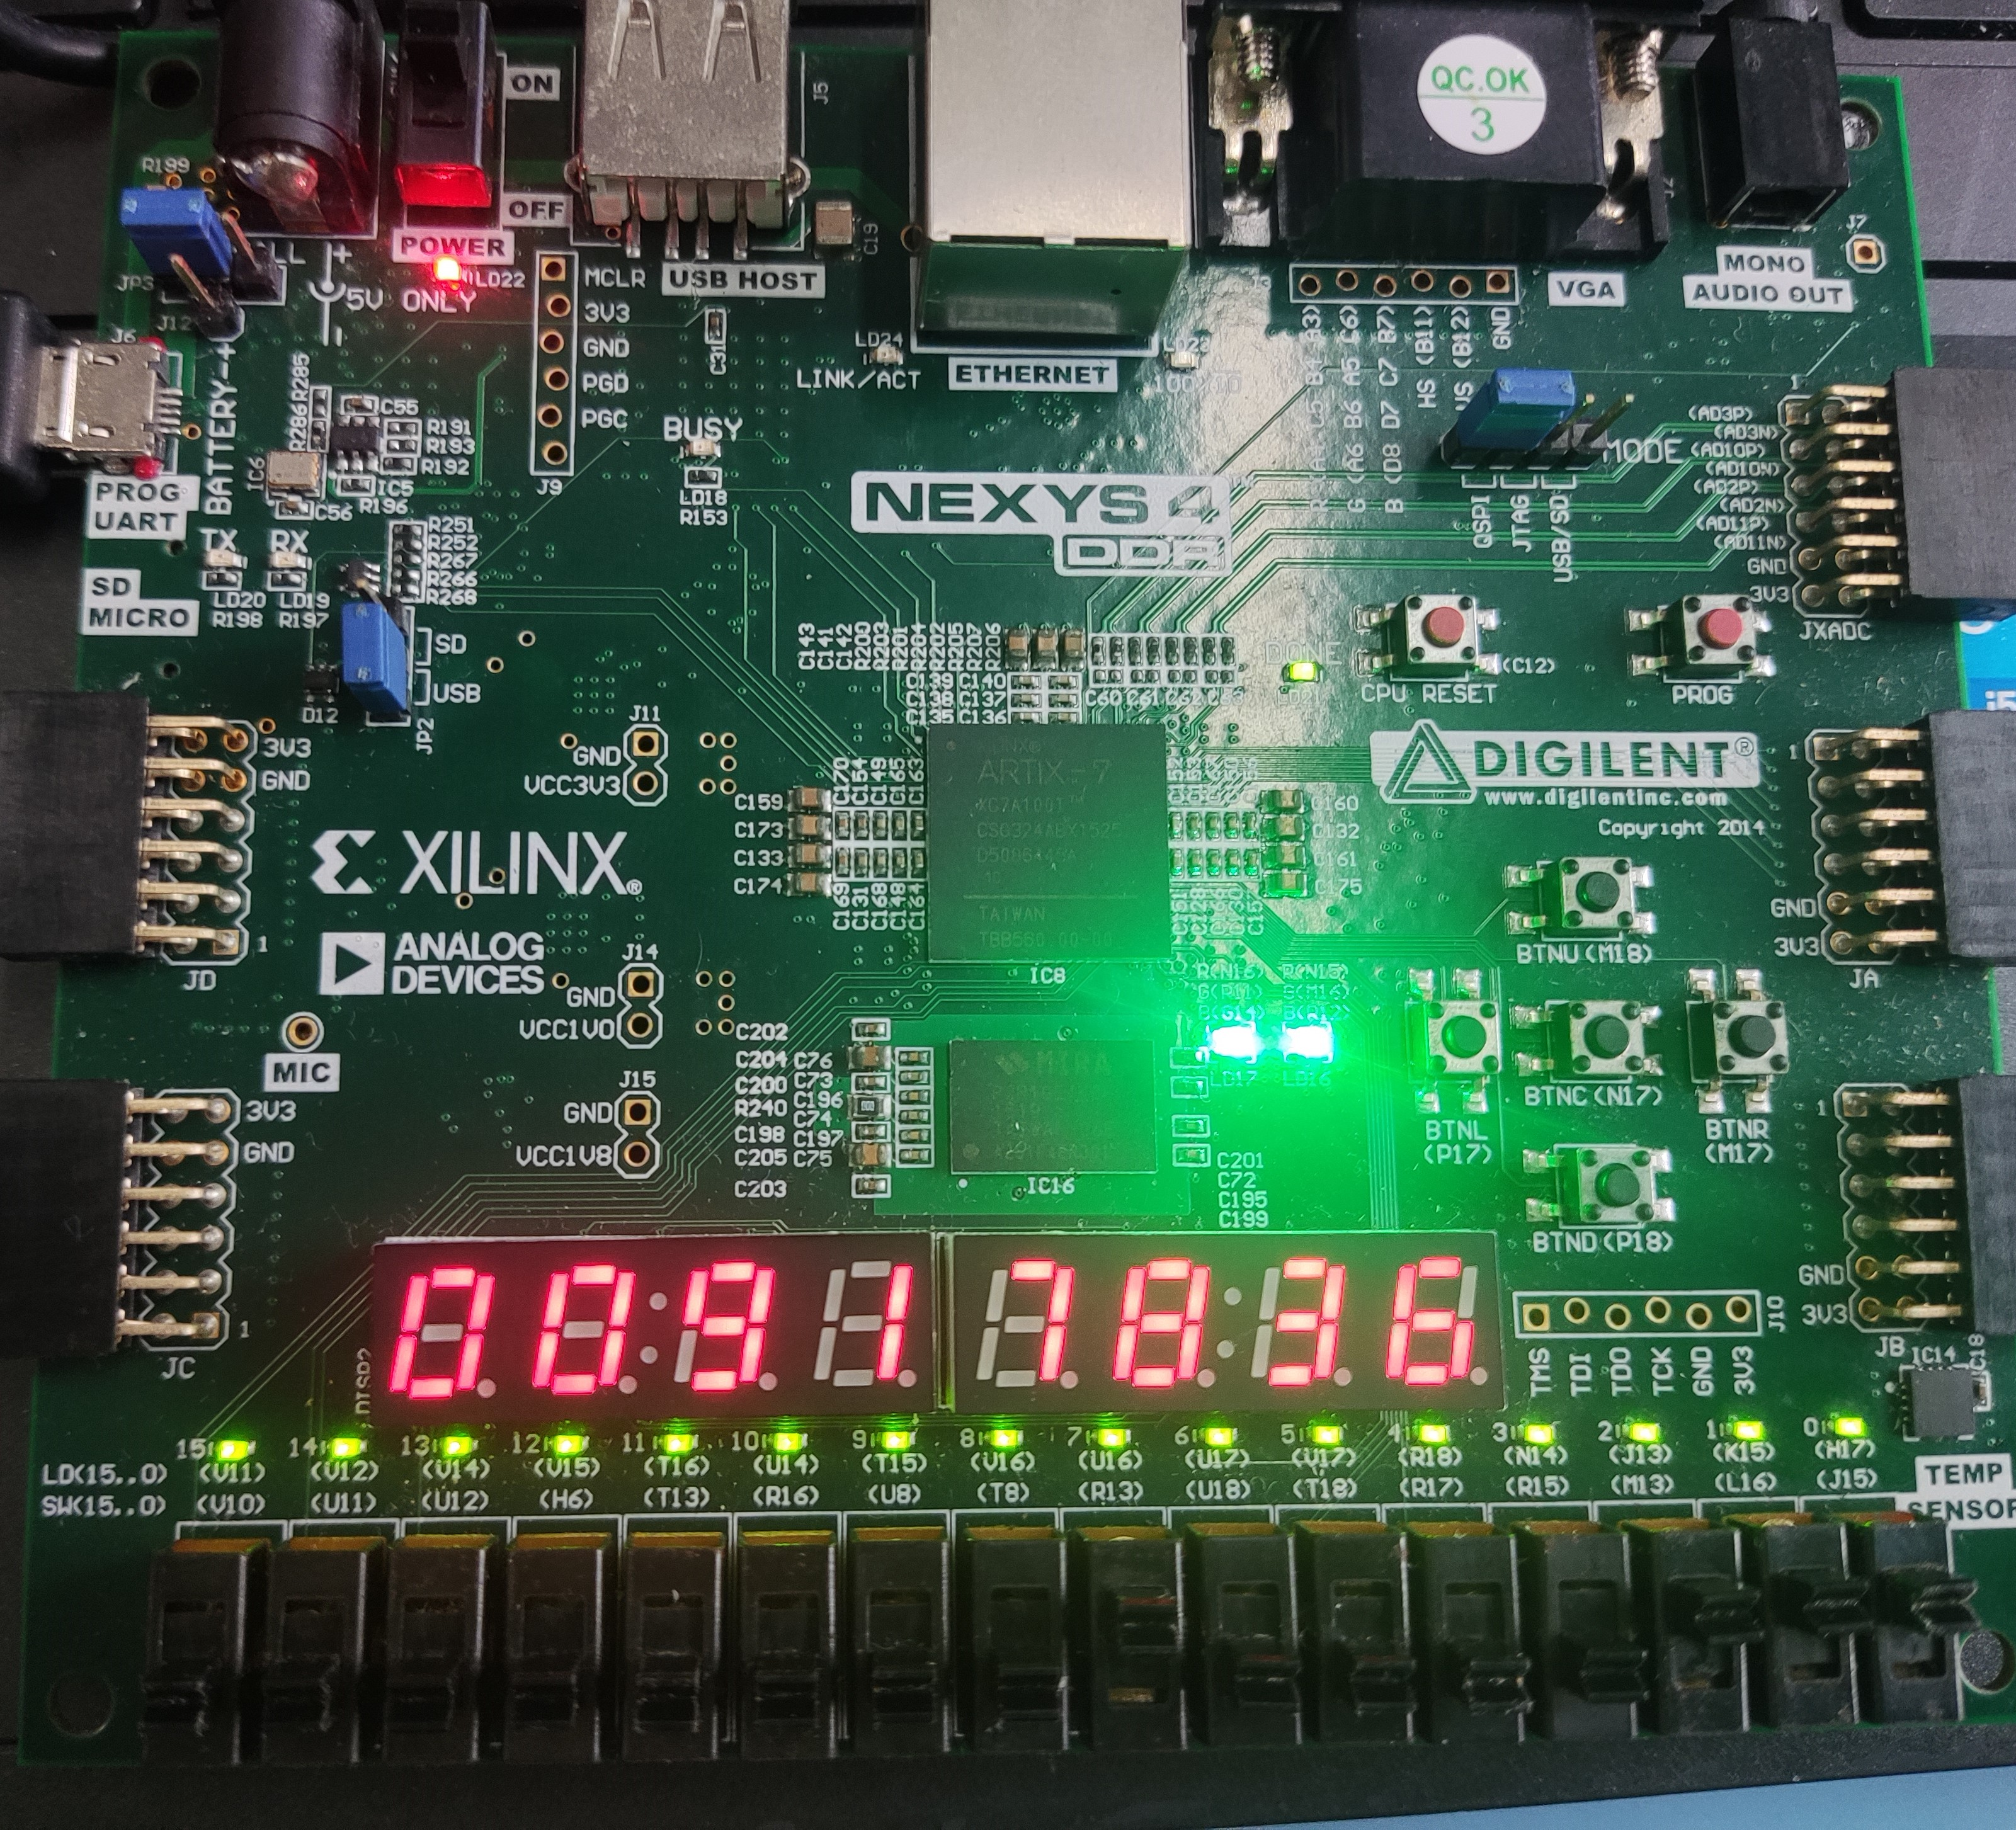
\includegraphics[width=0.7\textwidth]{image/per6.jpg}
    \caption{quicksort 性能测试得分}
    \label{fig:per6}
\end{figure}
\begin{figure}[htbp]
    \centering
    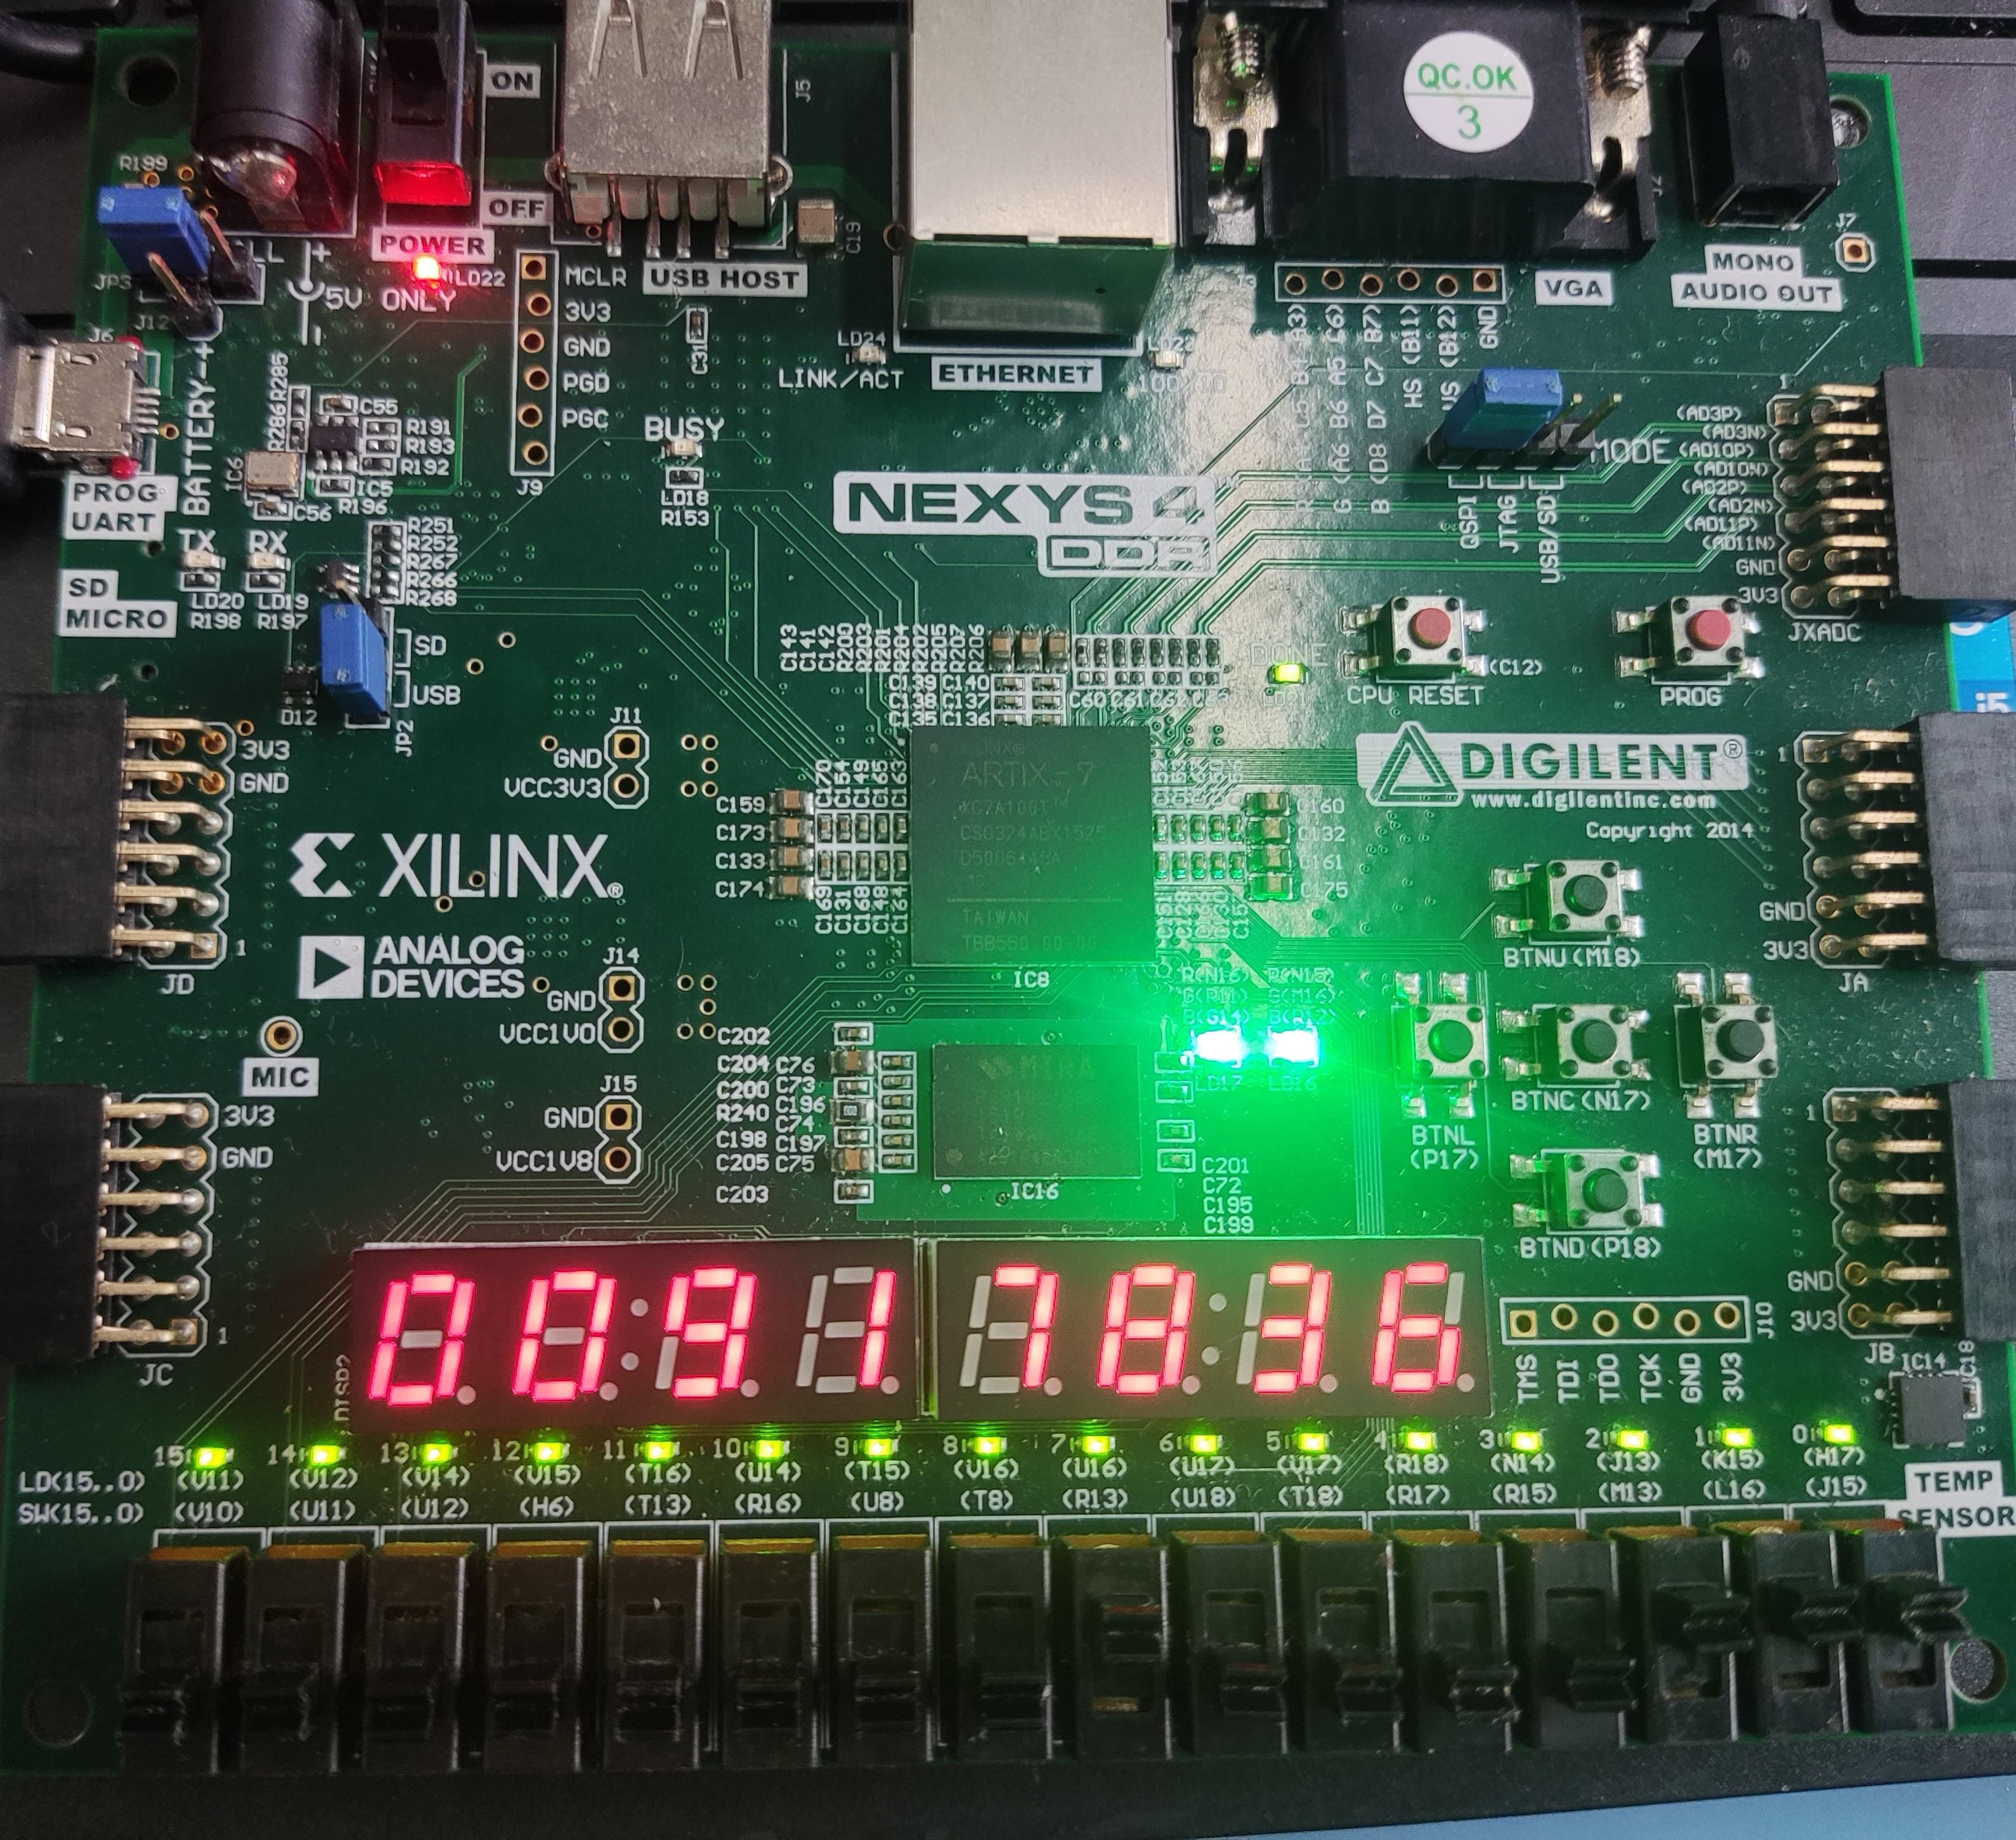
\includegraphics[width=0.7\textwidth]{image/per7.jpg}
    \caption{selectsort 性能测试得分}
    \label{fig:per7}
\end{figure}
\begin{figure}[htbp]
    \centering
    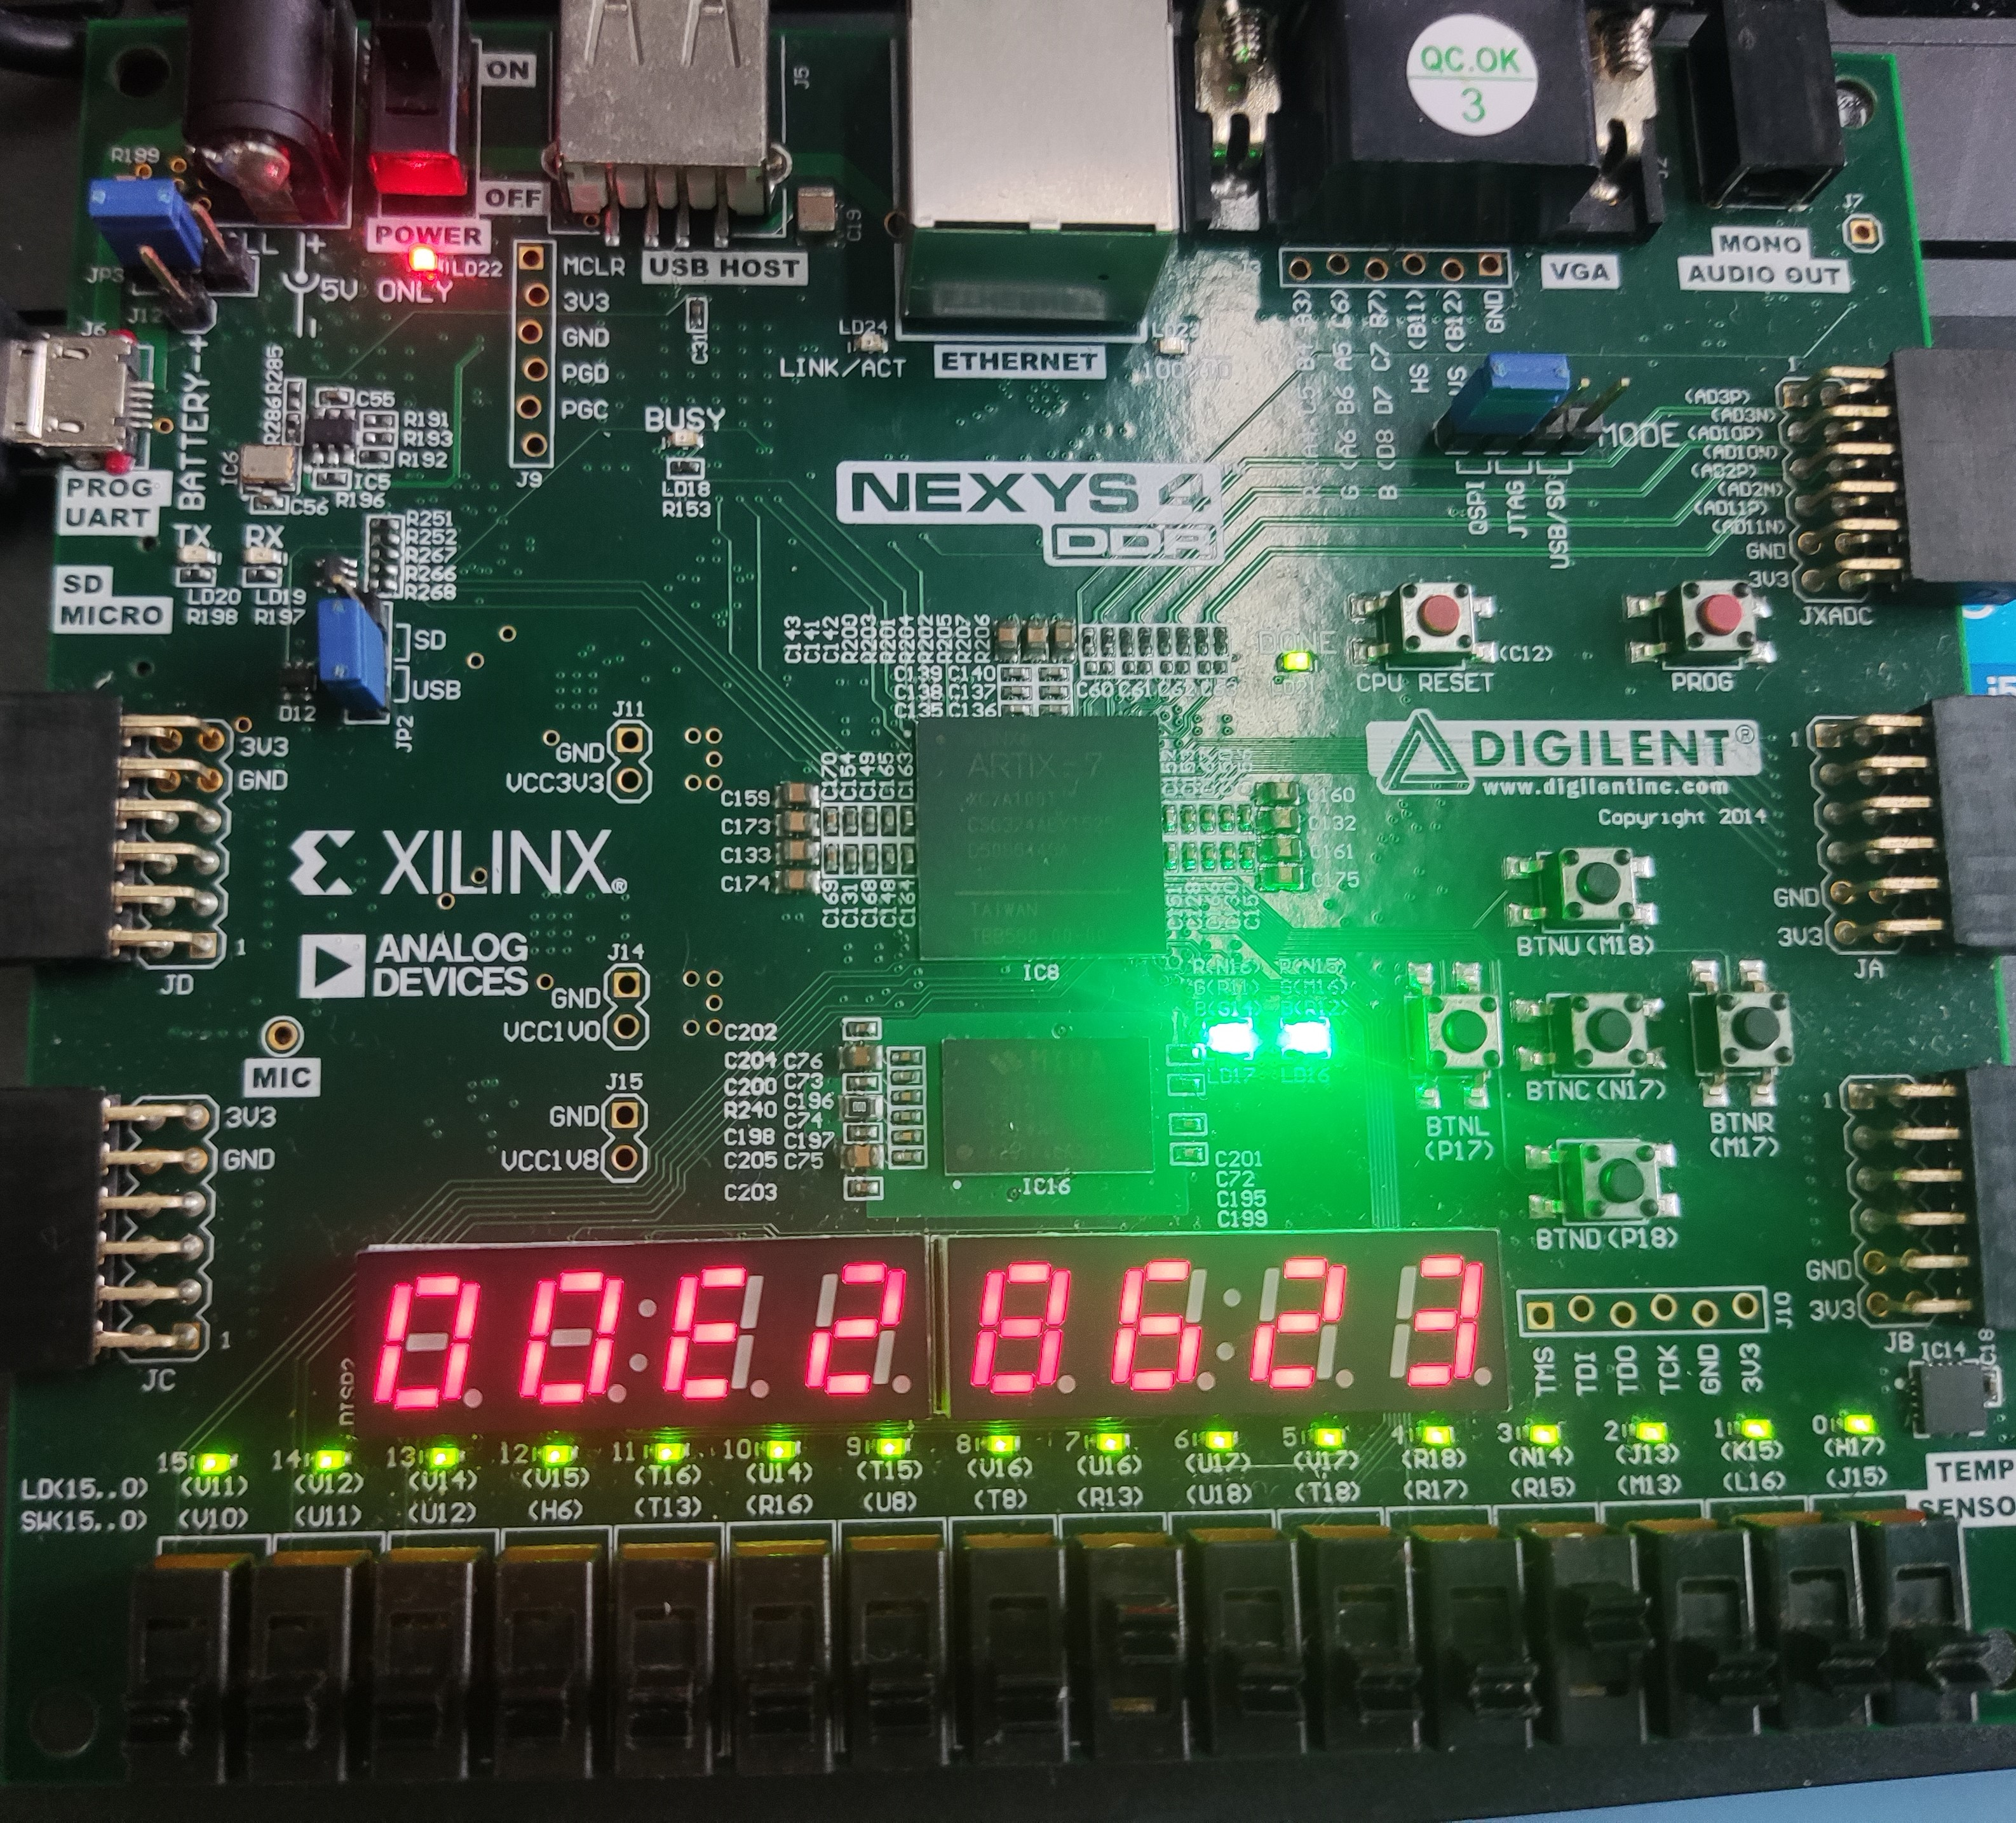
\includegraphics[width=0.7\textwidth]{image/per8.jpg}
    \caption{sha 性能测试得分}
    \label{fig:per8}
\end{figure}
\begin{figure}[htbp]
    \centering
    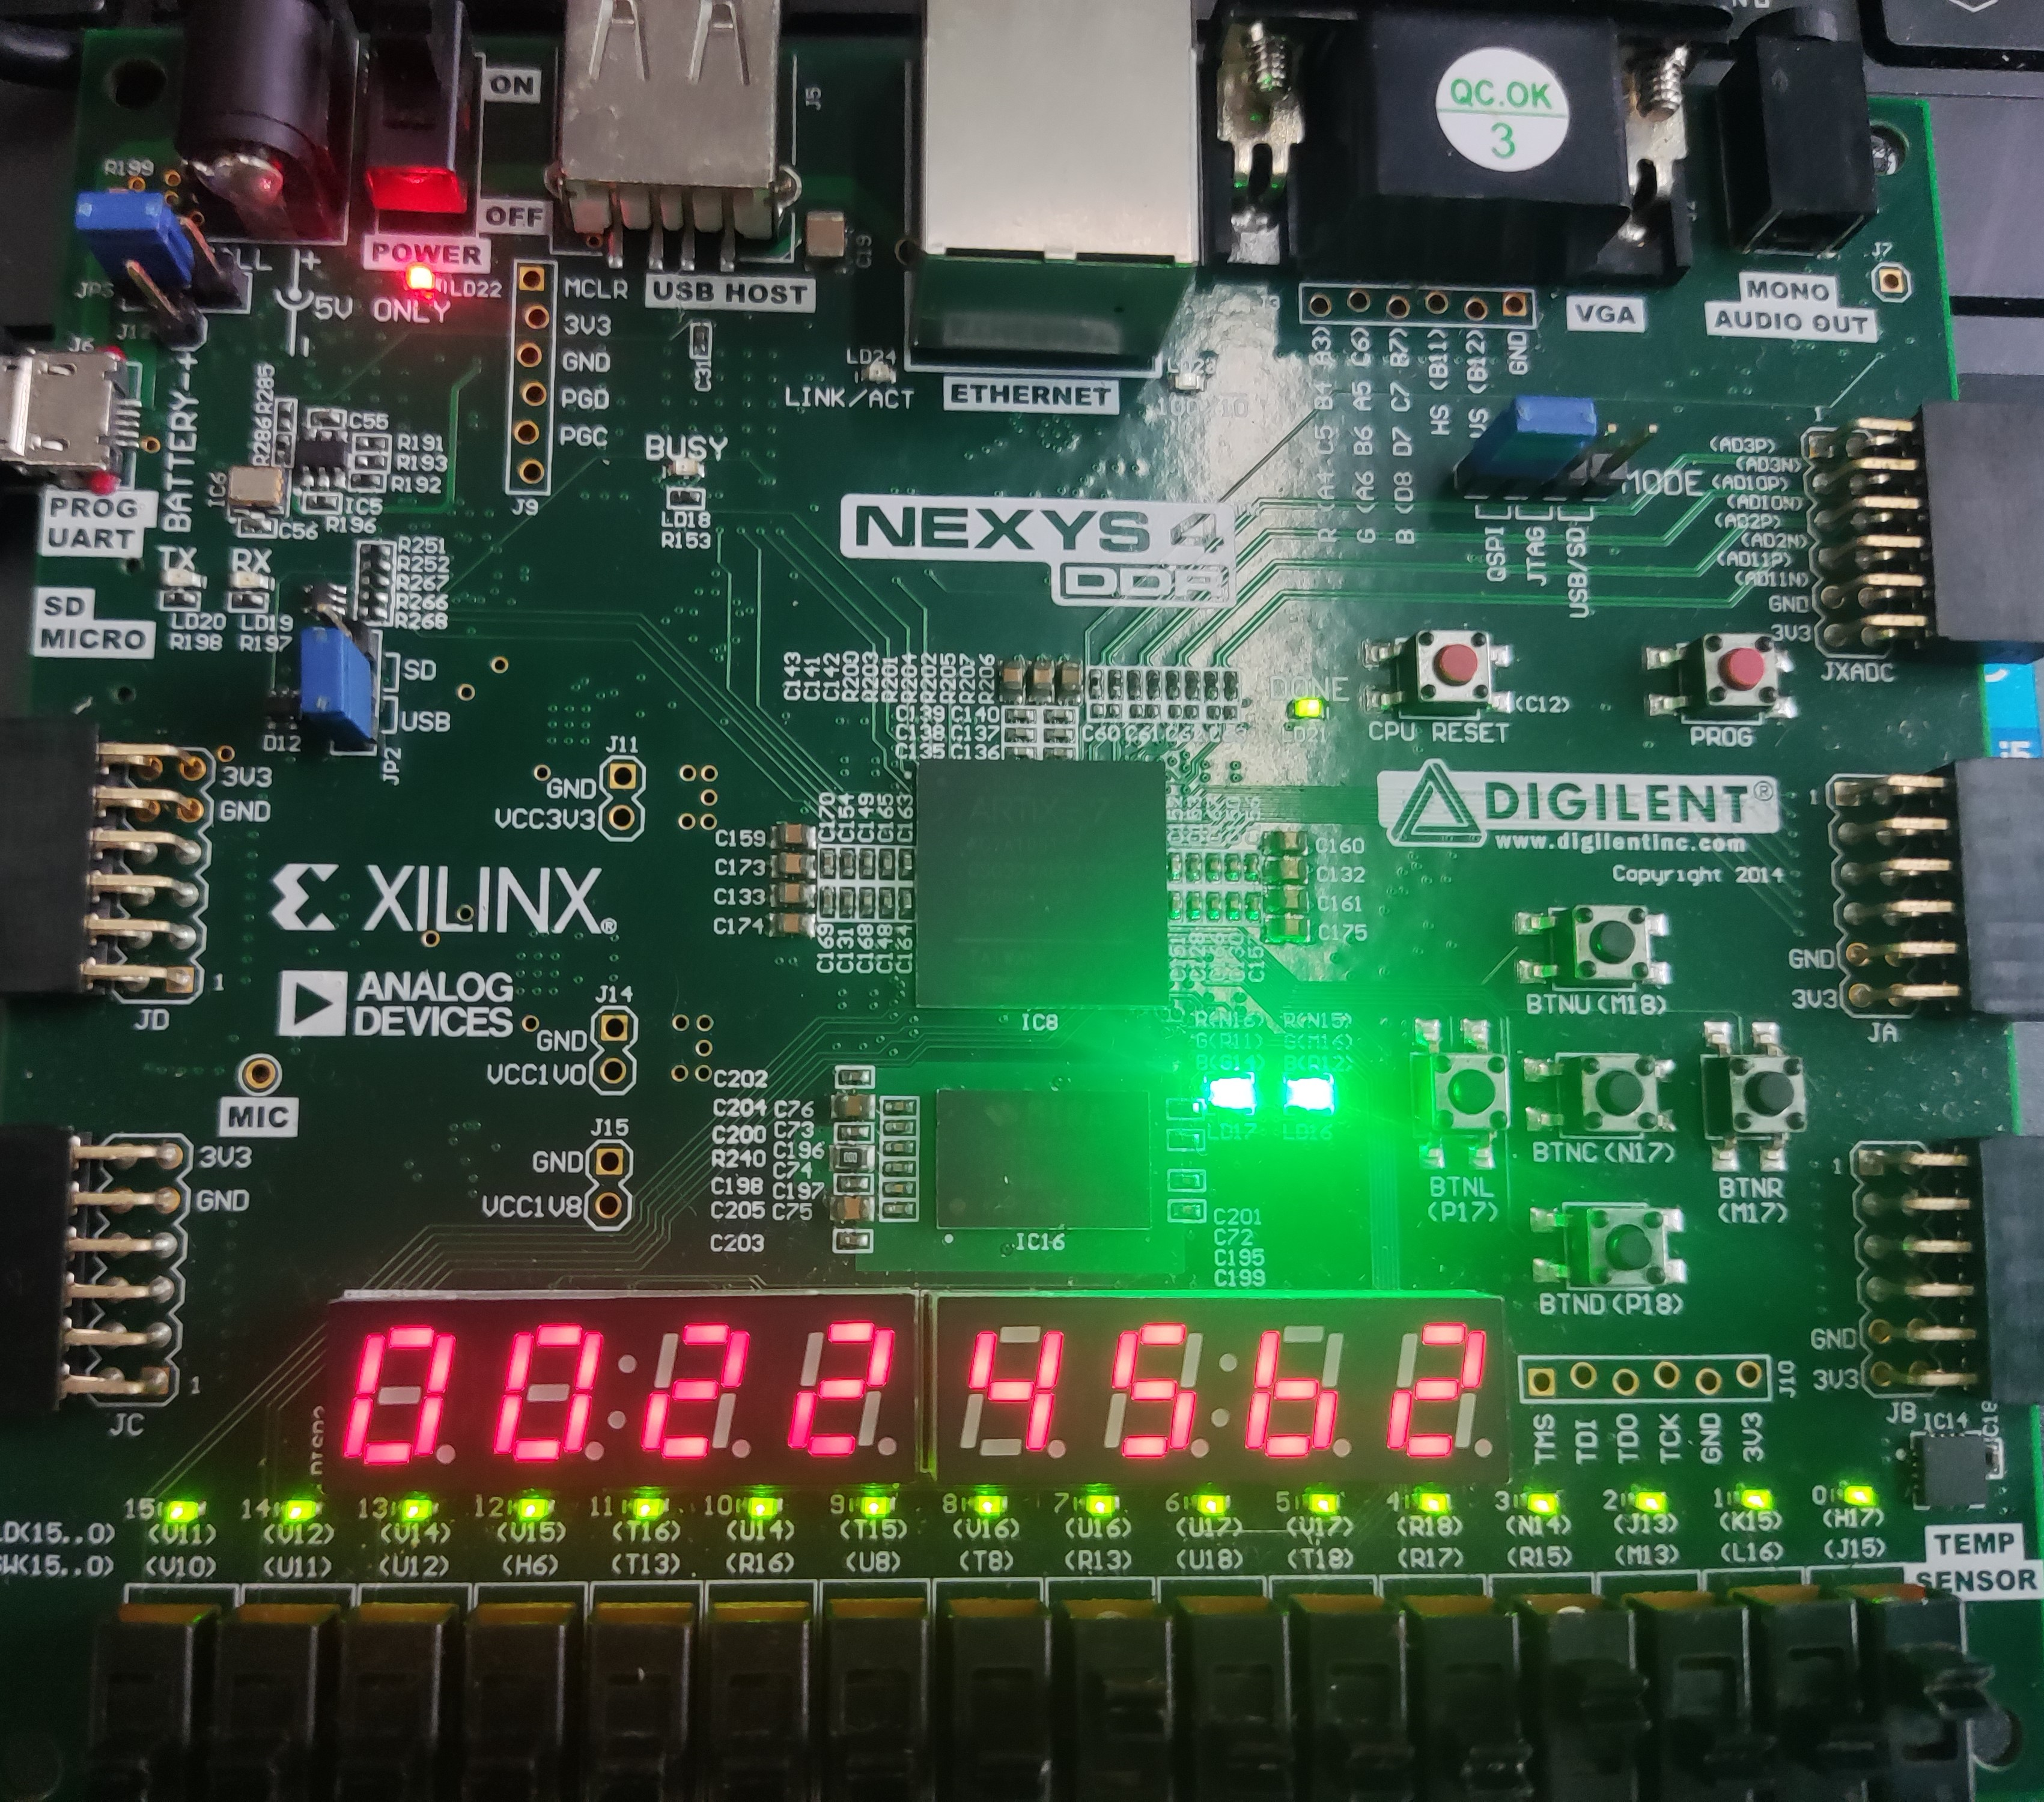
\includegraphics[width=0.7\textwidth]{image/per9.jpg}
    \caption{streamcopy 性能测试得分}
    \label{fig:per9}
\end{figure}
\begin{figure}[htbp]
    \centering
    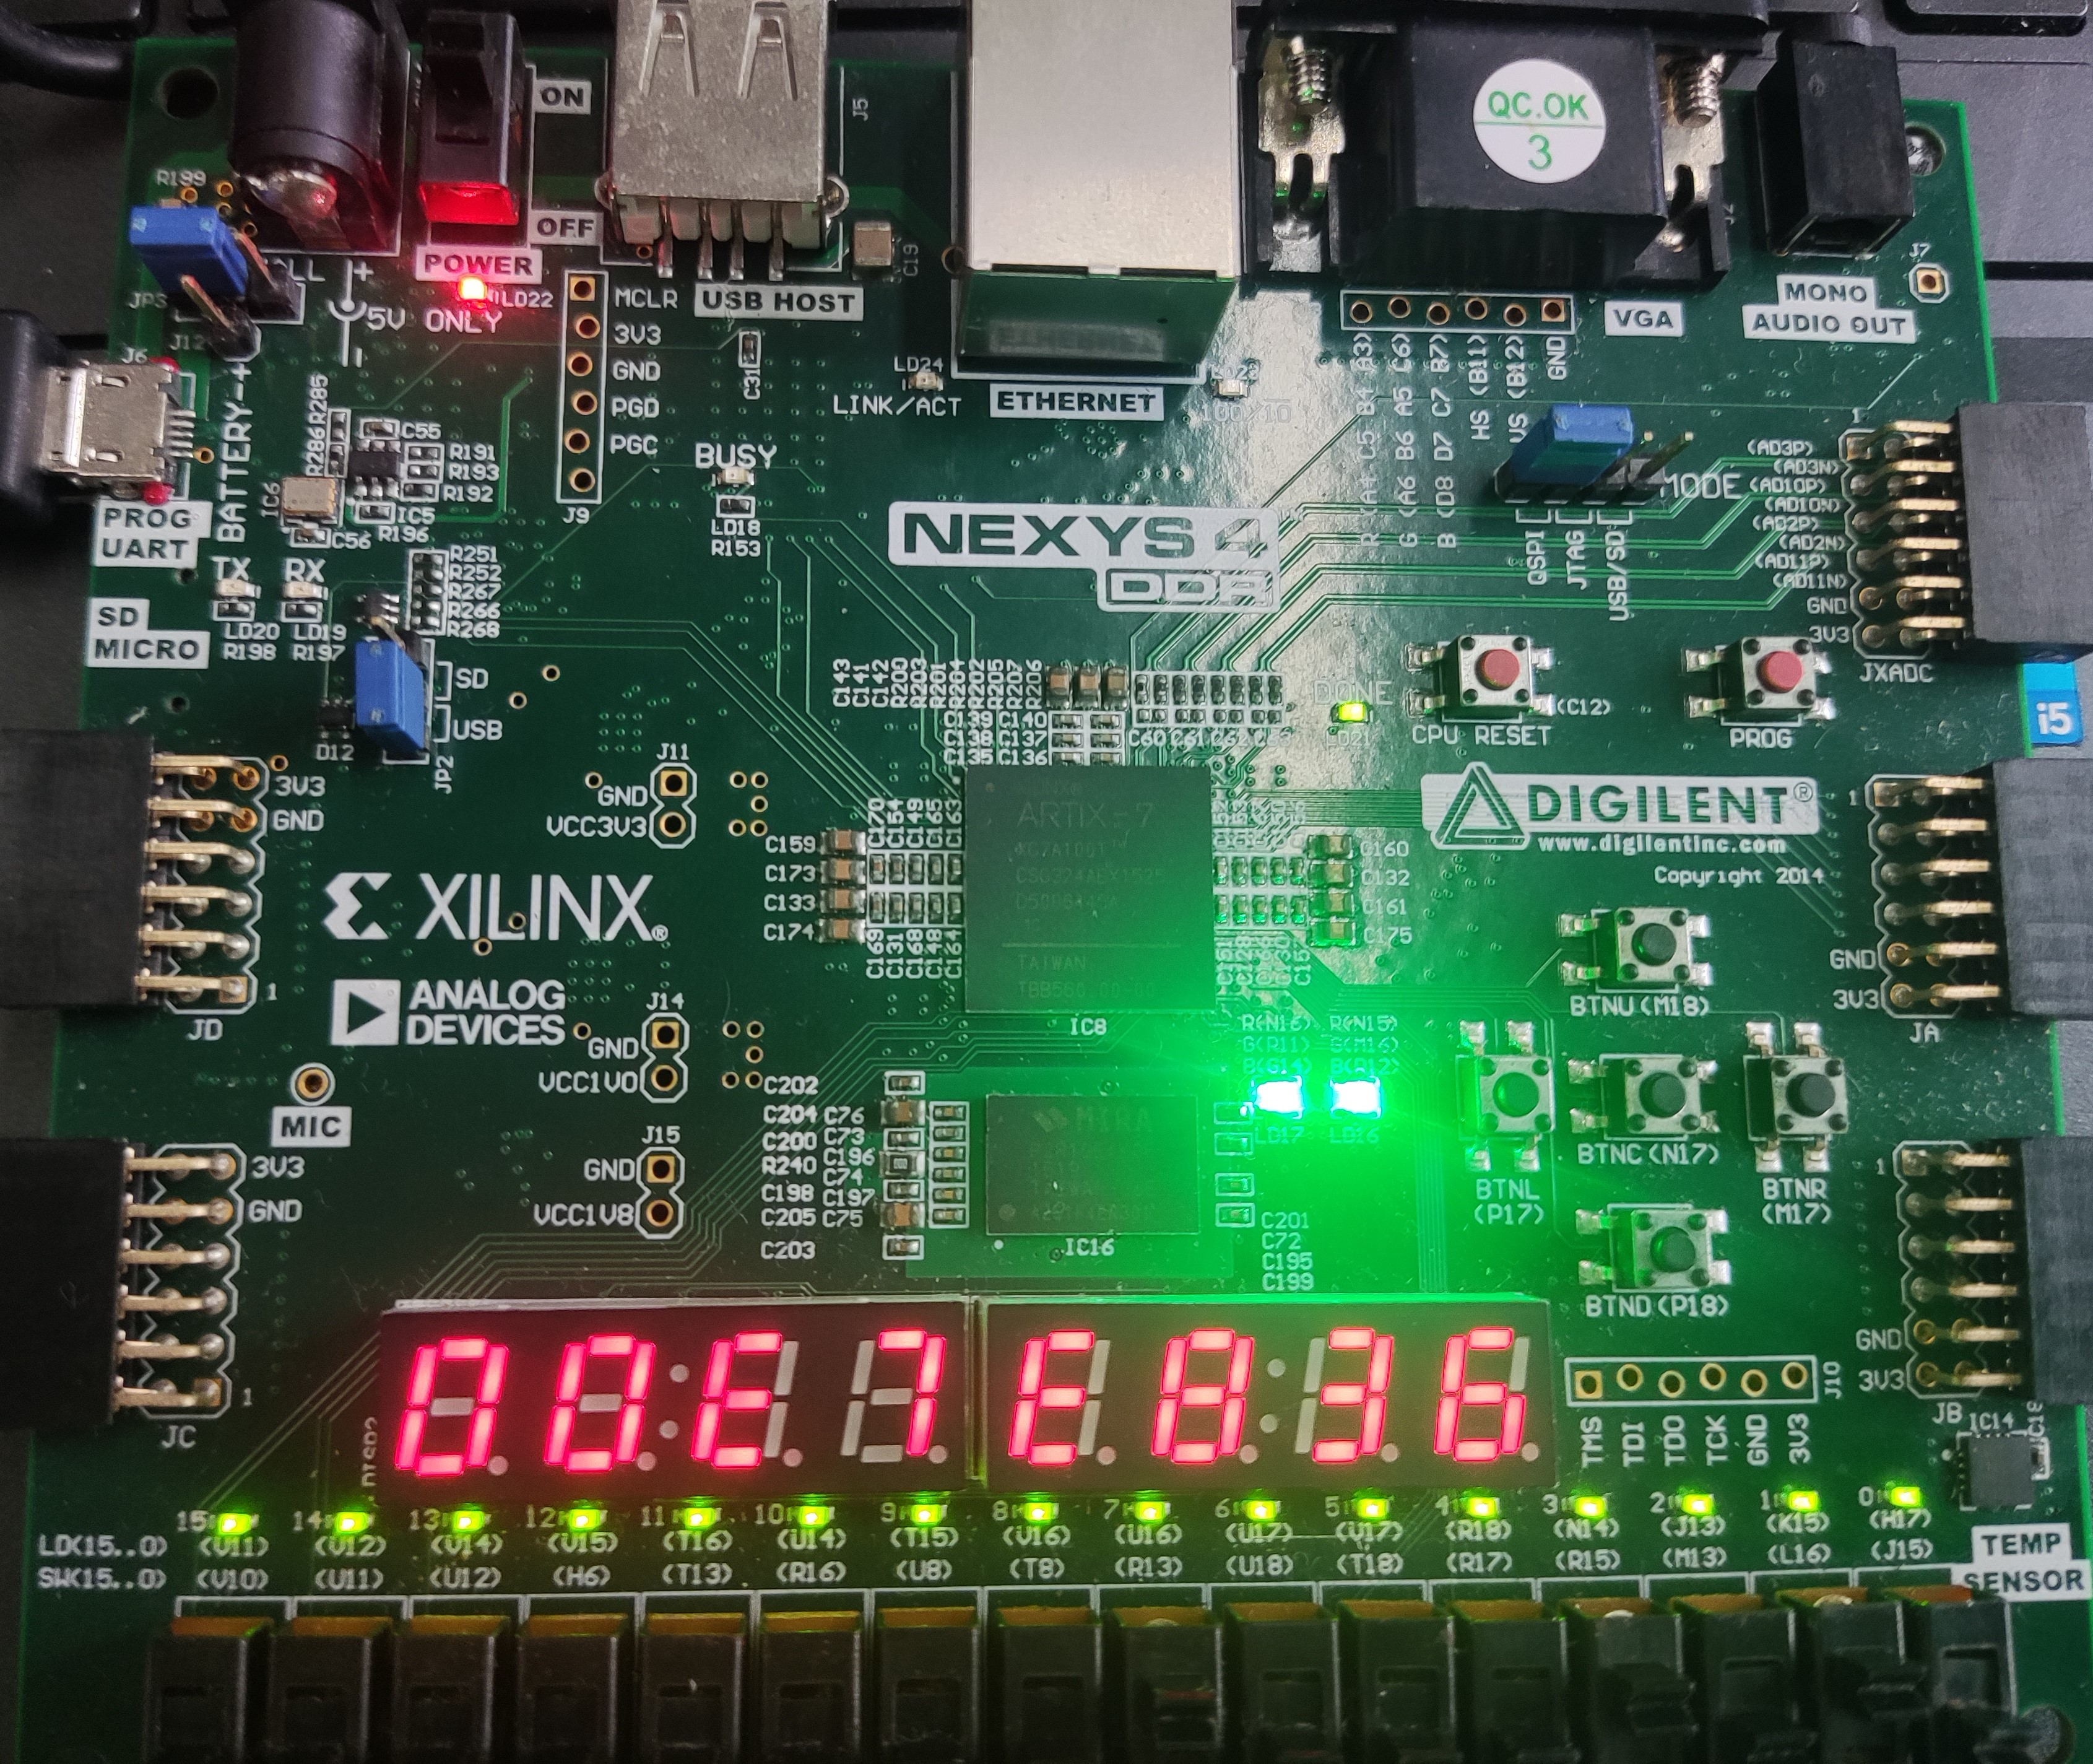
\includegraphics[width=0.7\textwidth]{image/per10.jpg}
    \caption{stringsearch 性能测试得分}
    \label{fig:per10}
\end{figure}
\newpage{}